%%%%%%%%%%%%%%%%%%%%%%%%%%%%%%%%%%%%%%%%%%%%%%%%%%%%%%%%%%
% # Appendix: Acceptability Judgment Task Results
%%%%%%%%%%%%%%%%%%%%%%%%%%%%%%%%%%%%%%%%%%%%%%%%%%%%%%%%%%

\chapter{Acceptability Judgment Task Results}\label{app-results-ajt}

\vspace{-3pt}

%========================================================%
\section{By-group rating patterns}\label{app-ajt-rating}
%========================================================%

% ORC Means
% \DTLloaddb{dt-ajt-rating}{../analysis/tables/ajt_rating.csv}
% \ExplSyntaxOn
% \tl_clear:N \tblrbody
% \tl_build_begin:N \tblrbody
% \DTLforeach[\equal{\study}{ORC}]{dt-ajt-rating}{\study=study,\coli=Pairing,\colii=Dependency,\coliii=Environment,\coliv=Mean,\colv=$CI$}{\tl_build_put_right:Ne \tblrbody {\exp_not:V \coli & \exp_not:V \colii & \exp_not:V \coliii & \exp_not:V \coliv & \exp_not:V \colv\\}}
% \tl_build_end:N \tblrbody
% \ExplSyntaxOff
% \begin{longtblr}[caption={Mean ratings in the ORC acceptability judgment task}, label={tblr:app-orc-ajt-rating}, expand=\tblrbody, remark{Note} = {EE~= ENS in English; KE~= KLE in English; ME~= MLE in English; KK~= KLE in Korean; MM~= MLE in Mandarin.}]{colspec={XXXX[r]X[r]}}\toprule
% Pairing & Dependency & Environment & Mean & 95\% \textit{CI}\\\midrule
% \tblrbody\bottomrule
% \end{longtblr}
% \vspace{-12pt}

% SRC Means
% \ExplSyntaxOn
% \tl_clear:N \tblrbody
% \tl_build_begin:N \tblrbody
% \DTLforeach[\equal{\study}{SRC}]{dt-ajt-rating}{\study=study,\coli=Pairing,\colii=Dependency,\coliii=Environment,\coliv=Mean,\colv=$CI$}{\tl_build_put_right:Ne \tblrbody {\exp_not:V \coli & \exp_not:V \colii & \exp_not:V \coliii & \exp_not:V \coliv & \exp_not:V \colv\\}}
% \tl_build_end:N \tblrbody
% \ExplSyntaxOff
% \begin{longtblr}[caption={Mean ratings in the SRC acceptability judgment task}, label={tblr:app-src-ajt-rating}, expand=\tblrbody, remark{Note} = {EE~= ENS in English; KE~= KLE in English; ME~= MLE in English; KK~= KLE in Korean; MM~= MLE in Mandarin.}]{colspec={XXXX[r]X[r]}}\toprule
% Pairing & Dependency & Environment & Mean & 95\% \textit{CI}\\\midrule
% \tblrbody\bottomrule
% \end{longtblr}
% \vspace{-12pt}

% ORC Figure
% \begin{figure}
% \caption{Mean ratings in the ORC acceptability judgment tasks} \label{fig:app-orc-ajt-rating}
% \raggedright\setstretch{1}
% 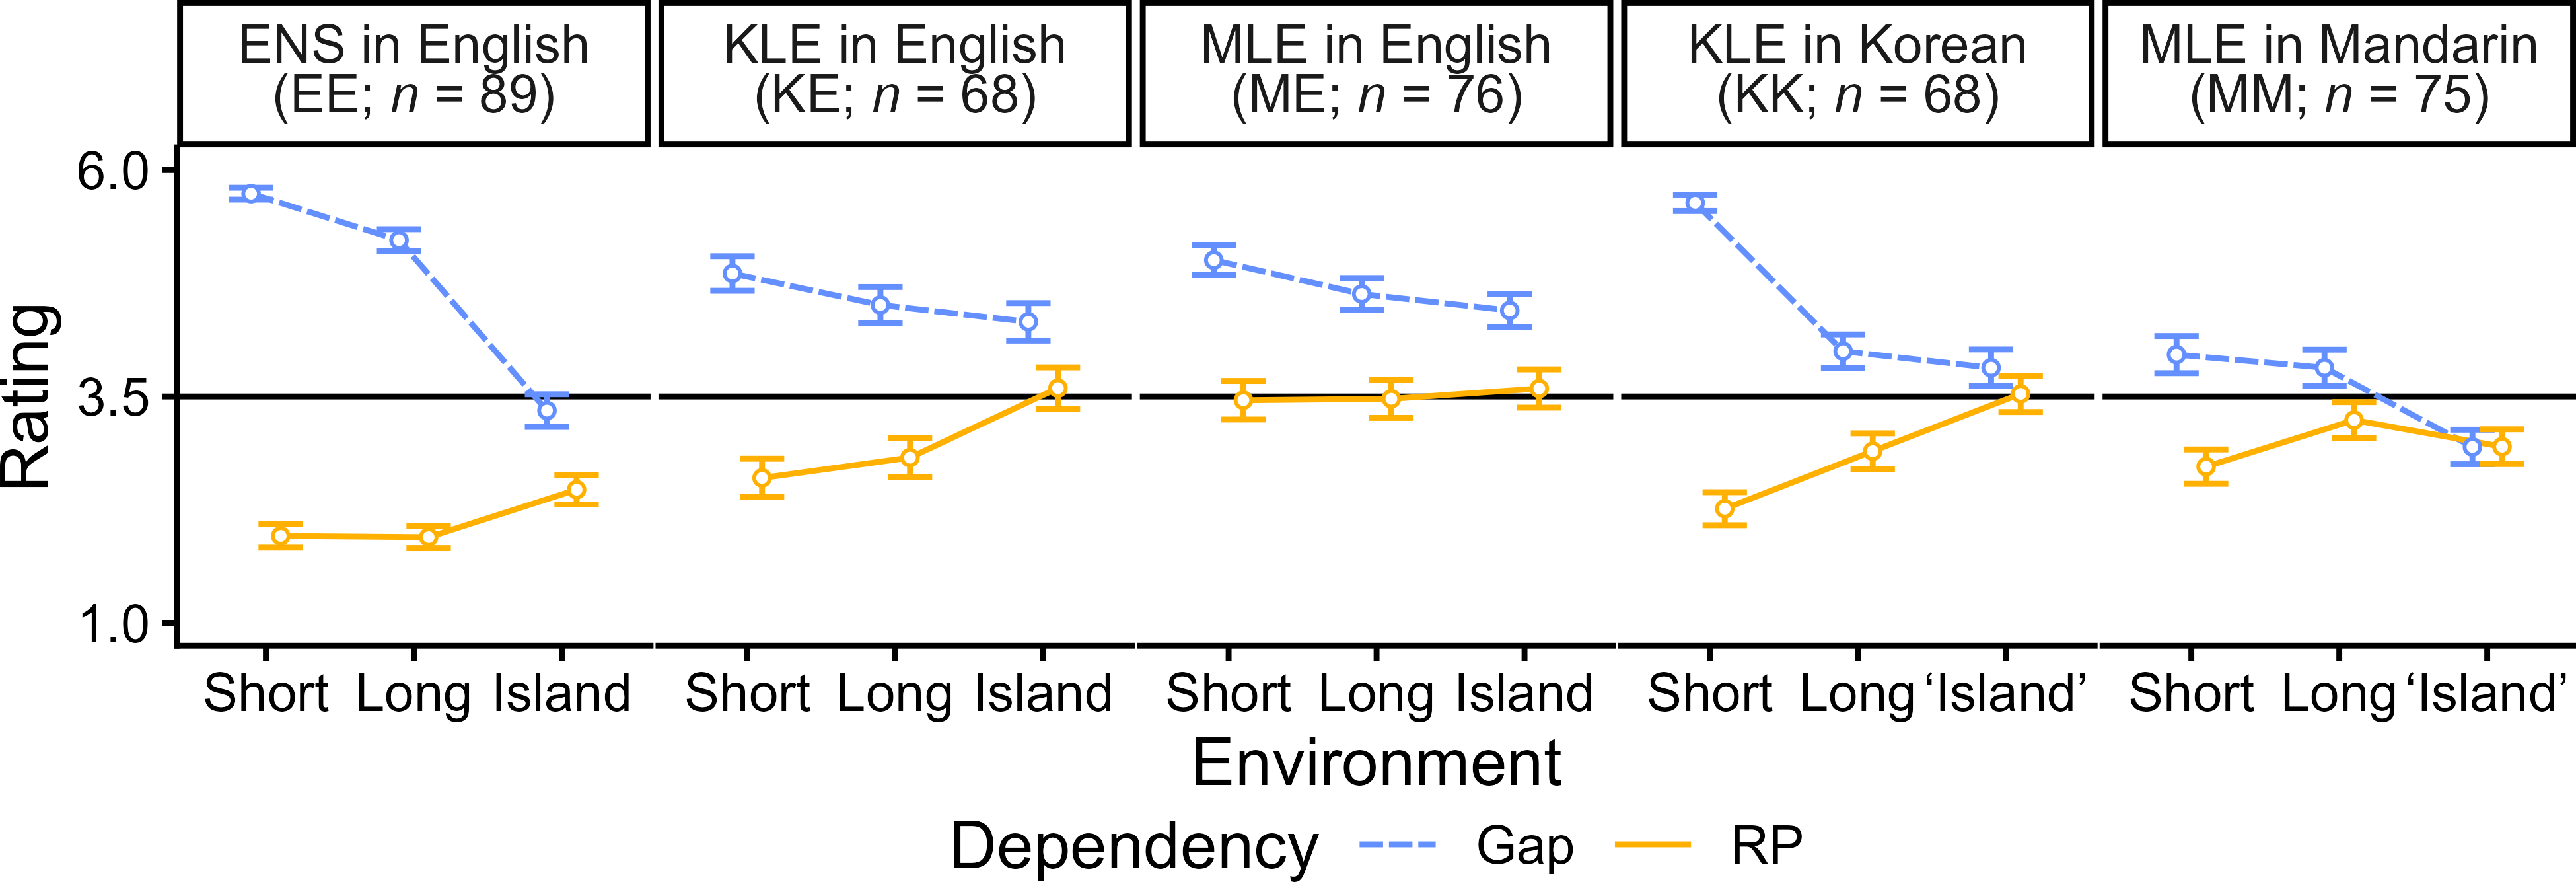
\includegraphics{../analysis/plots/orc_ajt_rating.png}
% \textit{Note}. Horizontal line marks midpoint on ratings scale; error bars are 95\% \textit{CI}s.
% \vspace{-12pt}
% \end{figure}

% SRC Figure
% \begin{figure}
% \caption{Mean ratings in the SRC acceptability judgment tasks} \label{fig:app-src-ajt-rating}
% \raggedright\setstretch{1}
% 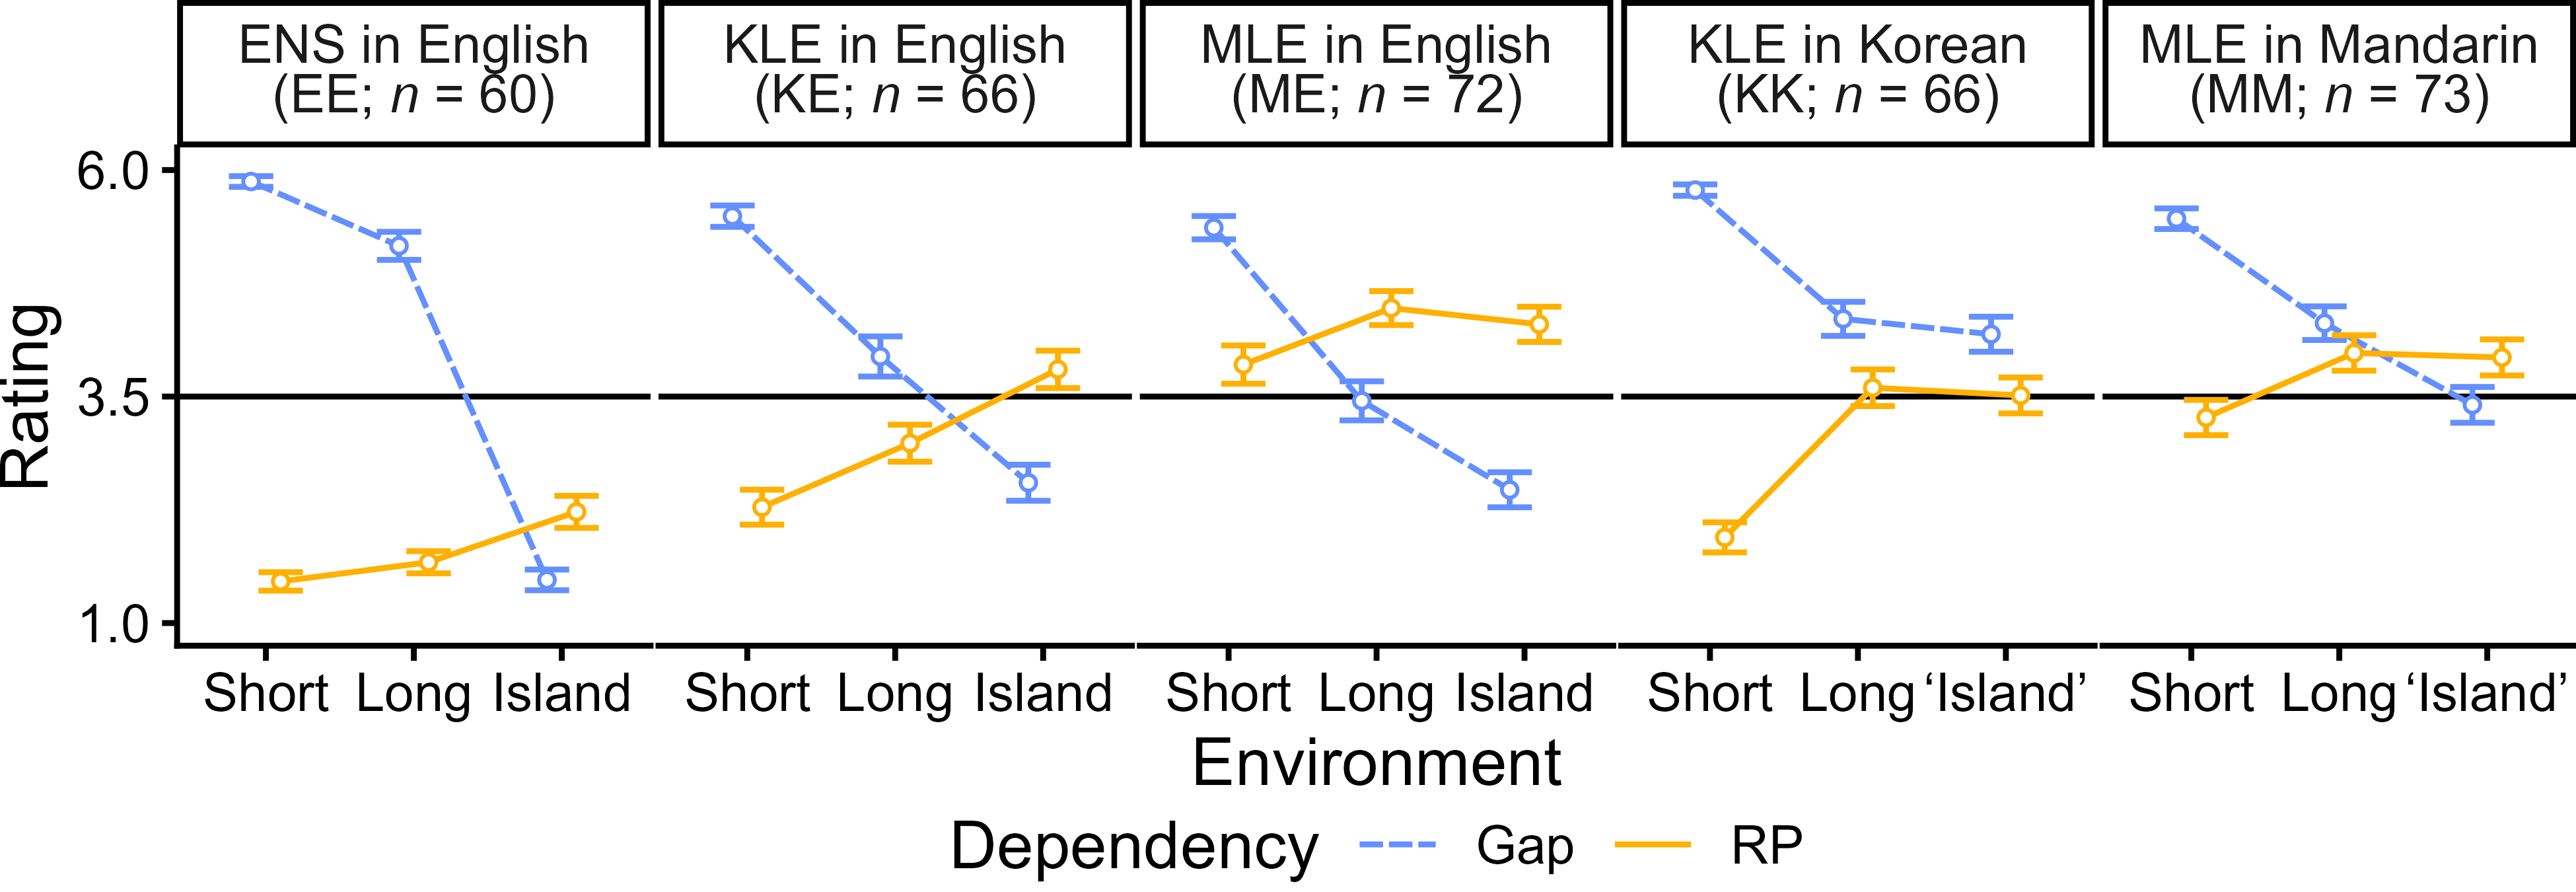
\includegraphics{../analysis/plots/src_ajt_rating.png}
% \textit{Note}. Horizontal line marks midpoint on ratings scale; error bars are 95\% \textit{CI}s.
% \vspace{-12pt}
% \end{figure}

\vspace{-16pt}

% ORC Model
\DTLloaddb{dt-orc-ajt-rating-model}{../analysis/tables/orc_ajt_rating_model.csv}
\ExplSyntaxOn
\tl_clear:N \tblrbody
\tl_build_begin:N \tblrbody
\DTLforeach{dt-orc-ajt-rating-model}{\coli=Parameter,\colii=Estimate,\coliii=$SE$,\coliv=$z$,\colv=$p$}{\tl_build_put_right:Ne \tblrbody {\exp_not:V \coli & \exp_not:V \colii & \exp_not:V \coliii & \exp_not:V \coliv & \exp_not:V \colv\\}}
\tl_build_end:N \tblrbody
\ExplSyntaxOff
\begin{longtblr}[caption={Summary of cumulative link mixed model on ratings in the ORC acceptability judgment task}, label={tblr:app-orc-ajt-rating-model}, expand=\tblrbody, remark{Note}={Model formula: Model formula: Rating \~{} Dependency * Environment * Pairing + (1 + Dependency + Environment | Participant) + (1 + Dependency + Environment + Pairing | Item).}]{colspec={lX[r]X[r]X[r]X[r]}}\toprule
Parameter & Estimate~($\hat{\beta}$) & \textit{SE} & $z$ & $p$\\\midrule
\tblrbody\bottomrule
\end{longtblr}
\vspace{-12pt}

% ; reference level: Gap + Short + EE; estimate unit: logit; intercept: grand mean

% SRC Posthoc
\begin{table}
\caption{Post-hoc tests for ratings in the ORC acceptability judgment task}\label{tab:app-orc-ajt-rating-posthoc}
\raggedright\setstretch{1}
\begin{tabularx}{\textwidth}{lXXYYYY}\toprule
Group & Environment & Contrast & Estimate~($\hat{\beta}$) & \textit{SE} & $z$ & $p$ \\\midrule
\csvreader[late after line=\\,late after last line=\\\bottomrule]
{../analysis/tables/orc_ajt_rating_posthoc.csv}{}{\csvcoli & \csvcolii & \csvcoliii & \csvcoliv & \csvcolv & \csvcolvi & \csvcolvii}
\end{tabularx}
\textit{Note}. Adjustment to $p$-values done via multiple $t$ method for 15 tests.
\vspace{-12pt}
\end{table}

% SRC Model
\DTLloaddb{dt-src-ajt-rating-model}{../analysis/tables/src_ajt_rating_model.csv}
\ExplSyntaxOn
\tl_clear:N \tblrbody
\tl_build_begin:N \tblrbody
\DTLforeach{dt-src-ajt-rating-model}{\coli=Parameter,\colii=Estimate,\coliii=$SE$,\coliv=$z$,\colv=$p$}{\tl_build_put_right:Ne \tblrbody {\exp_not:V \coli & \exp_not:V \colii & \exp_not:V \coliii & \exp_not:V \coliv & \exp_not:V \colv\\}}
\tl_build_end:N \tblrbody
\ExplSyntaxOff
\begin{longtblr}[caption={Summary of cumulative link mixed model on ratings in the SRC acceptability judgment task}, label={tblr:app-src-ajt-rating-model}, expand=\tblrbody, remark{Note}={Model formula: Model formula: Rating \~{} Dependency * Environment * Pairing + (1 + Dependency + Environment | Participant) + (1 + Dependency + Environment + Pairing | Item); reference level: Gap + Short + EE; estimate unit: logit; intercept: grand mean.}]{colspec={lX[r]X[r]X[r]X[r]}}\toprule
Parameter & Estimate~($\hat{\beta}$) & \textit{SE} & $z$ & $p$\\\midrule
\tblrbody\bottomrule
\end{longtblr}
\vspace{-12pt}

% SRC Posthoc
\begin{table}
\caption{Post-hoc tests for ratings in the SRC acceptability judgment task}\label{tab:app-src-ajt-rating-posthoc}
\raggedright\setstretch{1}
\begin{tabularx}{\textwidth}{lXXYYYY}\toprule
Group & Environment & Contrast & Estimate~($\hat{\beta}$) & \textit{SE} & $z$ & $p$ \\\midrule
\csvreader[late after line=\\,late after last line=\\\bottomrule]
{../analysis/tables/src_ajt_rating_posthoc.csv}{}{\csvcoli & \csvcolii & \csvcoliii & \csvcoliv & \csvcolv & \csvcolvi & \csvcolvii}
\end{tabularx}
\textit{Note}. Adjustment to $p$-values done via multiple $t$ method for 15 tests.
\end{table}

\newpage

%========================================================%
\section{L2 proficiency effects for by-group rating patterns}\label{app-ajt-rating-proficiency}
%========================================================%

% ORC Figure
% \begin{figure}
% \caption{Relationship between L2 proficiency and ratings in the ORC acceptability judgment task} \label{fig:app-orc-ajt-rating-proficiency}
% \raggedright\setstretch{1}
% 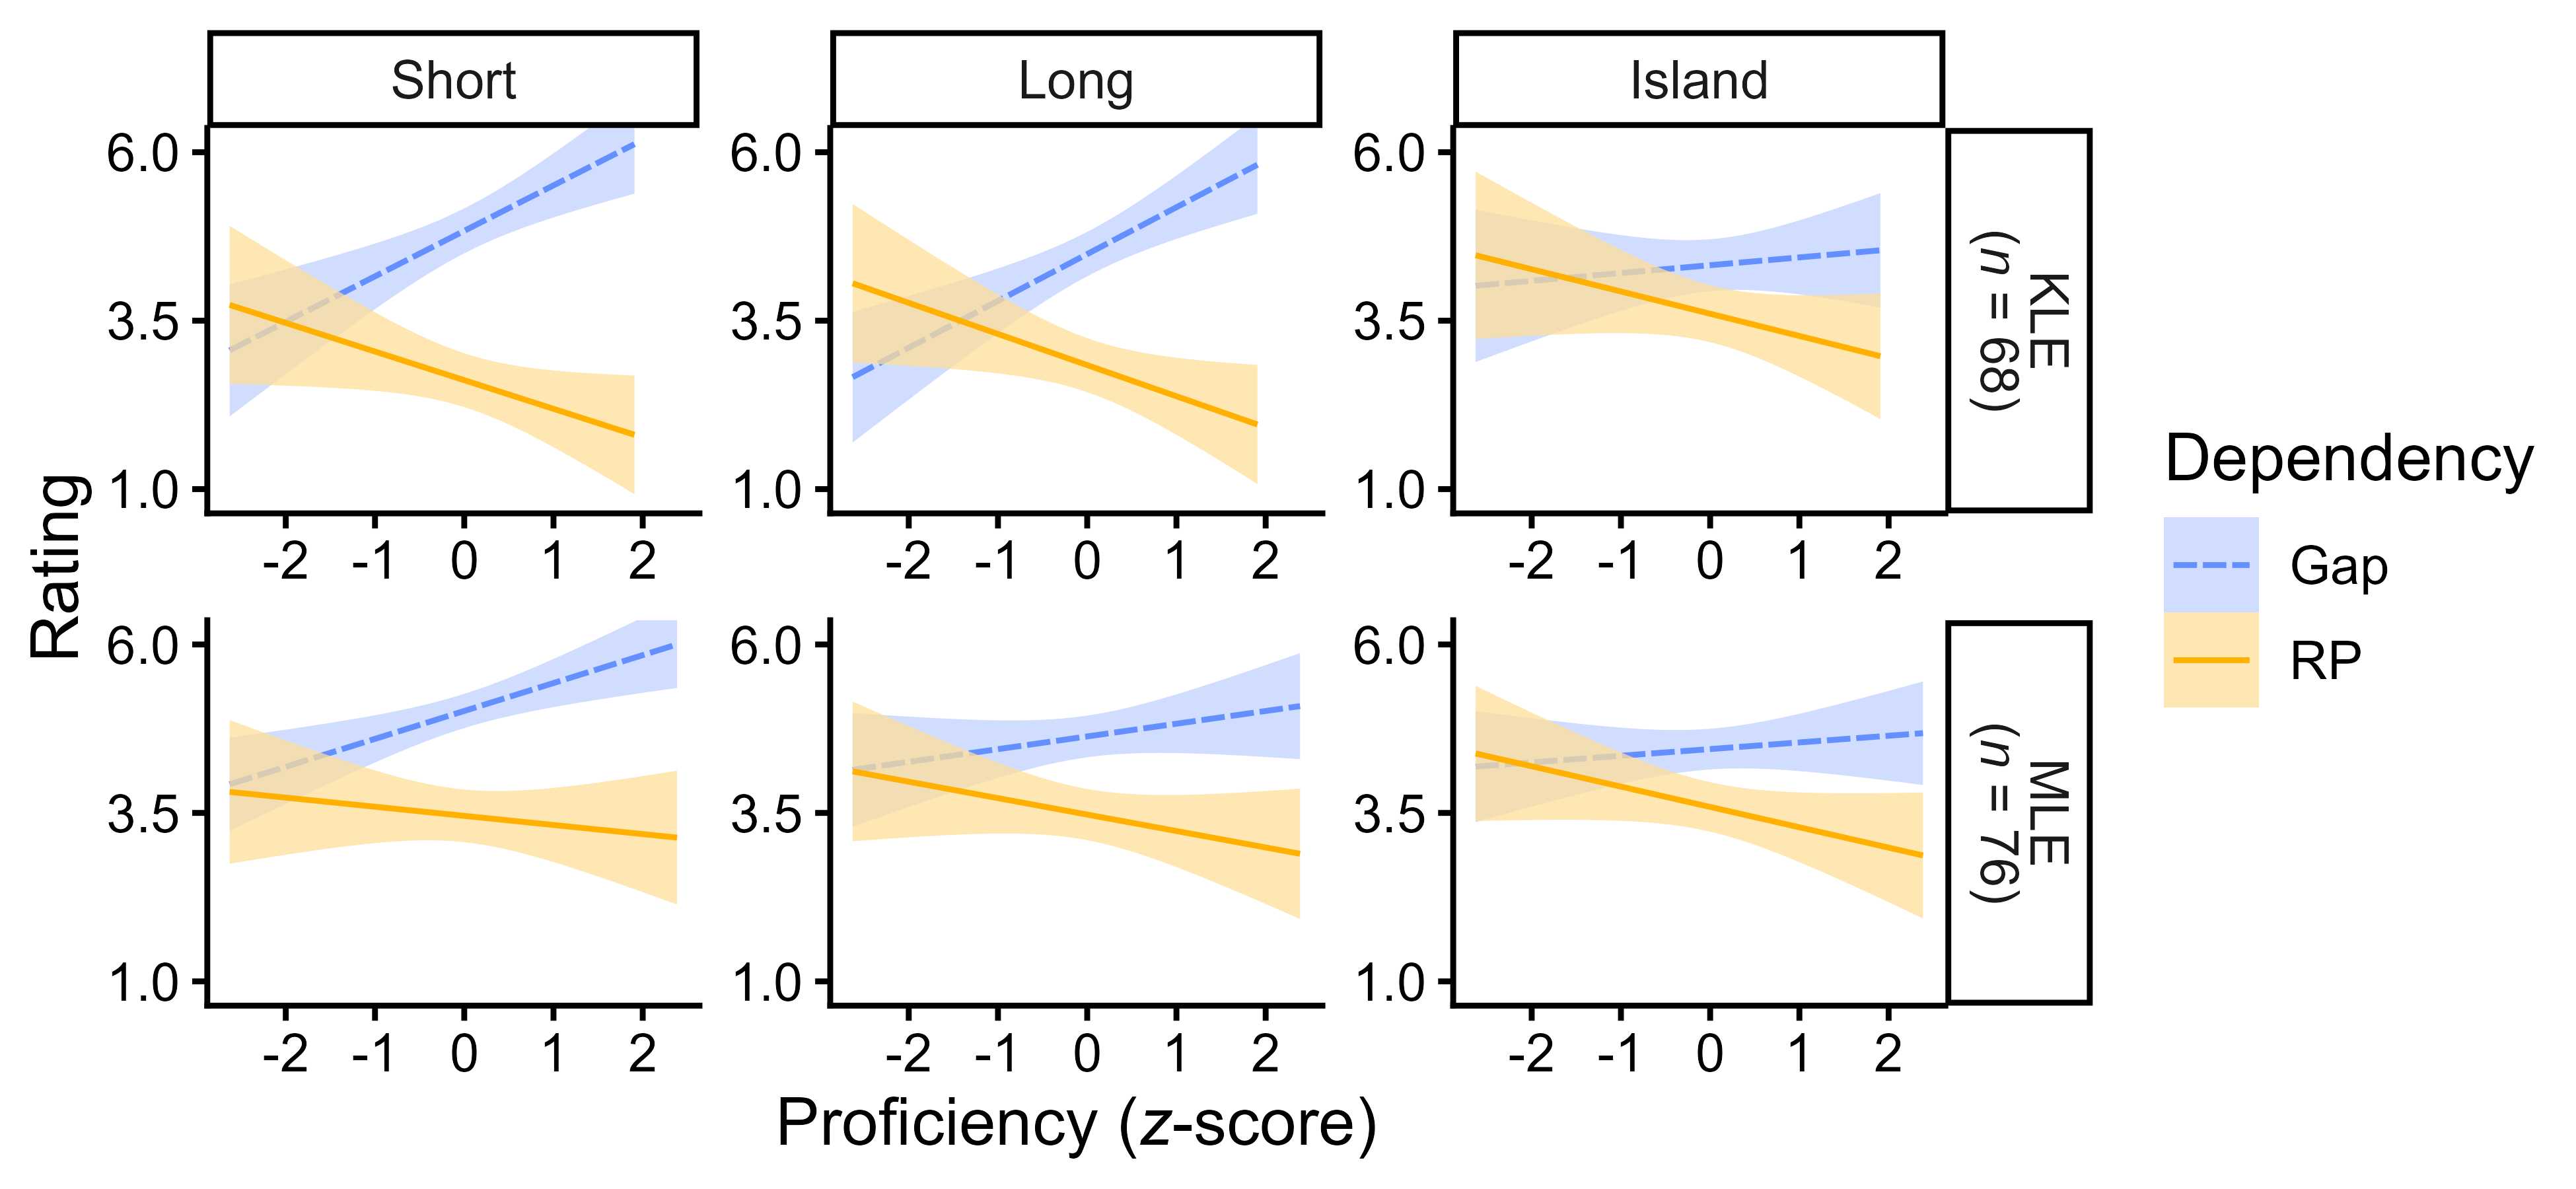
\includegraphics{../analysis/plots/orc_ajt_rating_proficiency.png}
% \textit{Note}. Shading indicates 95\% \textit{CI}s.
% \vspace{-12pt}
% \end{figure}

% SRC Figure
% \begin{figure}
% \caption{Relationship between L2 proficiency and ratings in the SRC acceptability judgment task} \label{fig:app-src-ajt-rating-proficiency}
% \raggedright\setstretch{1}
% 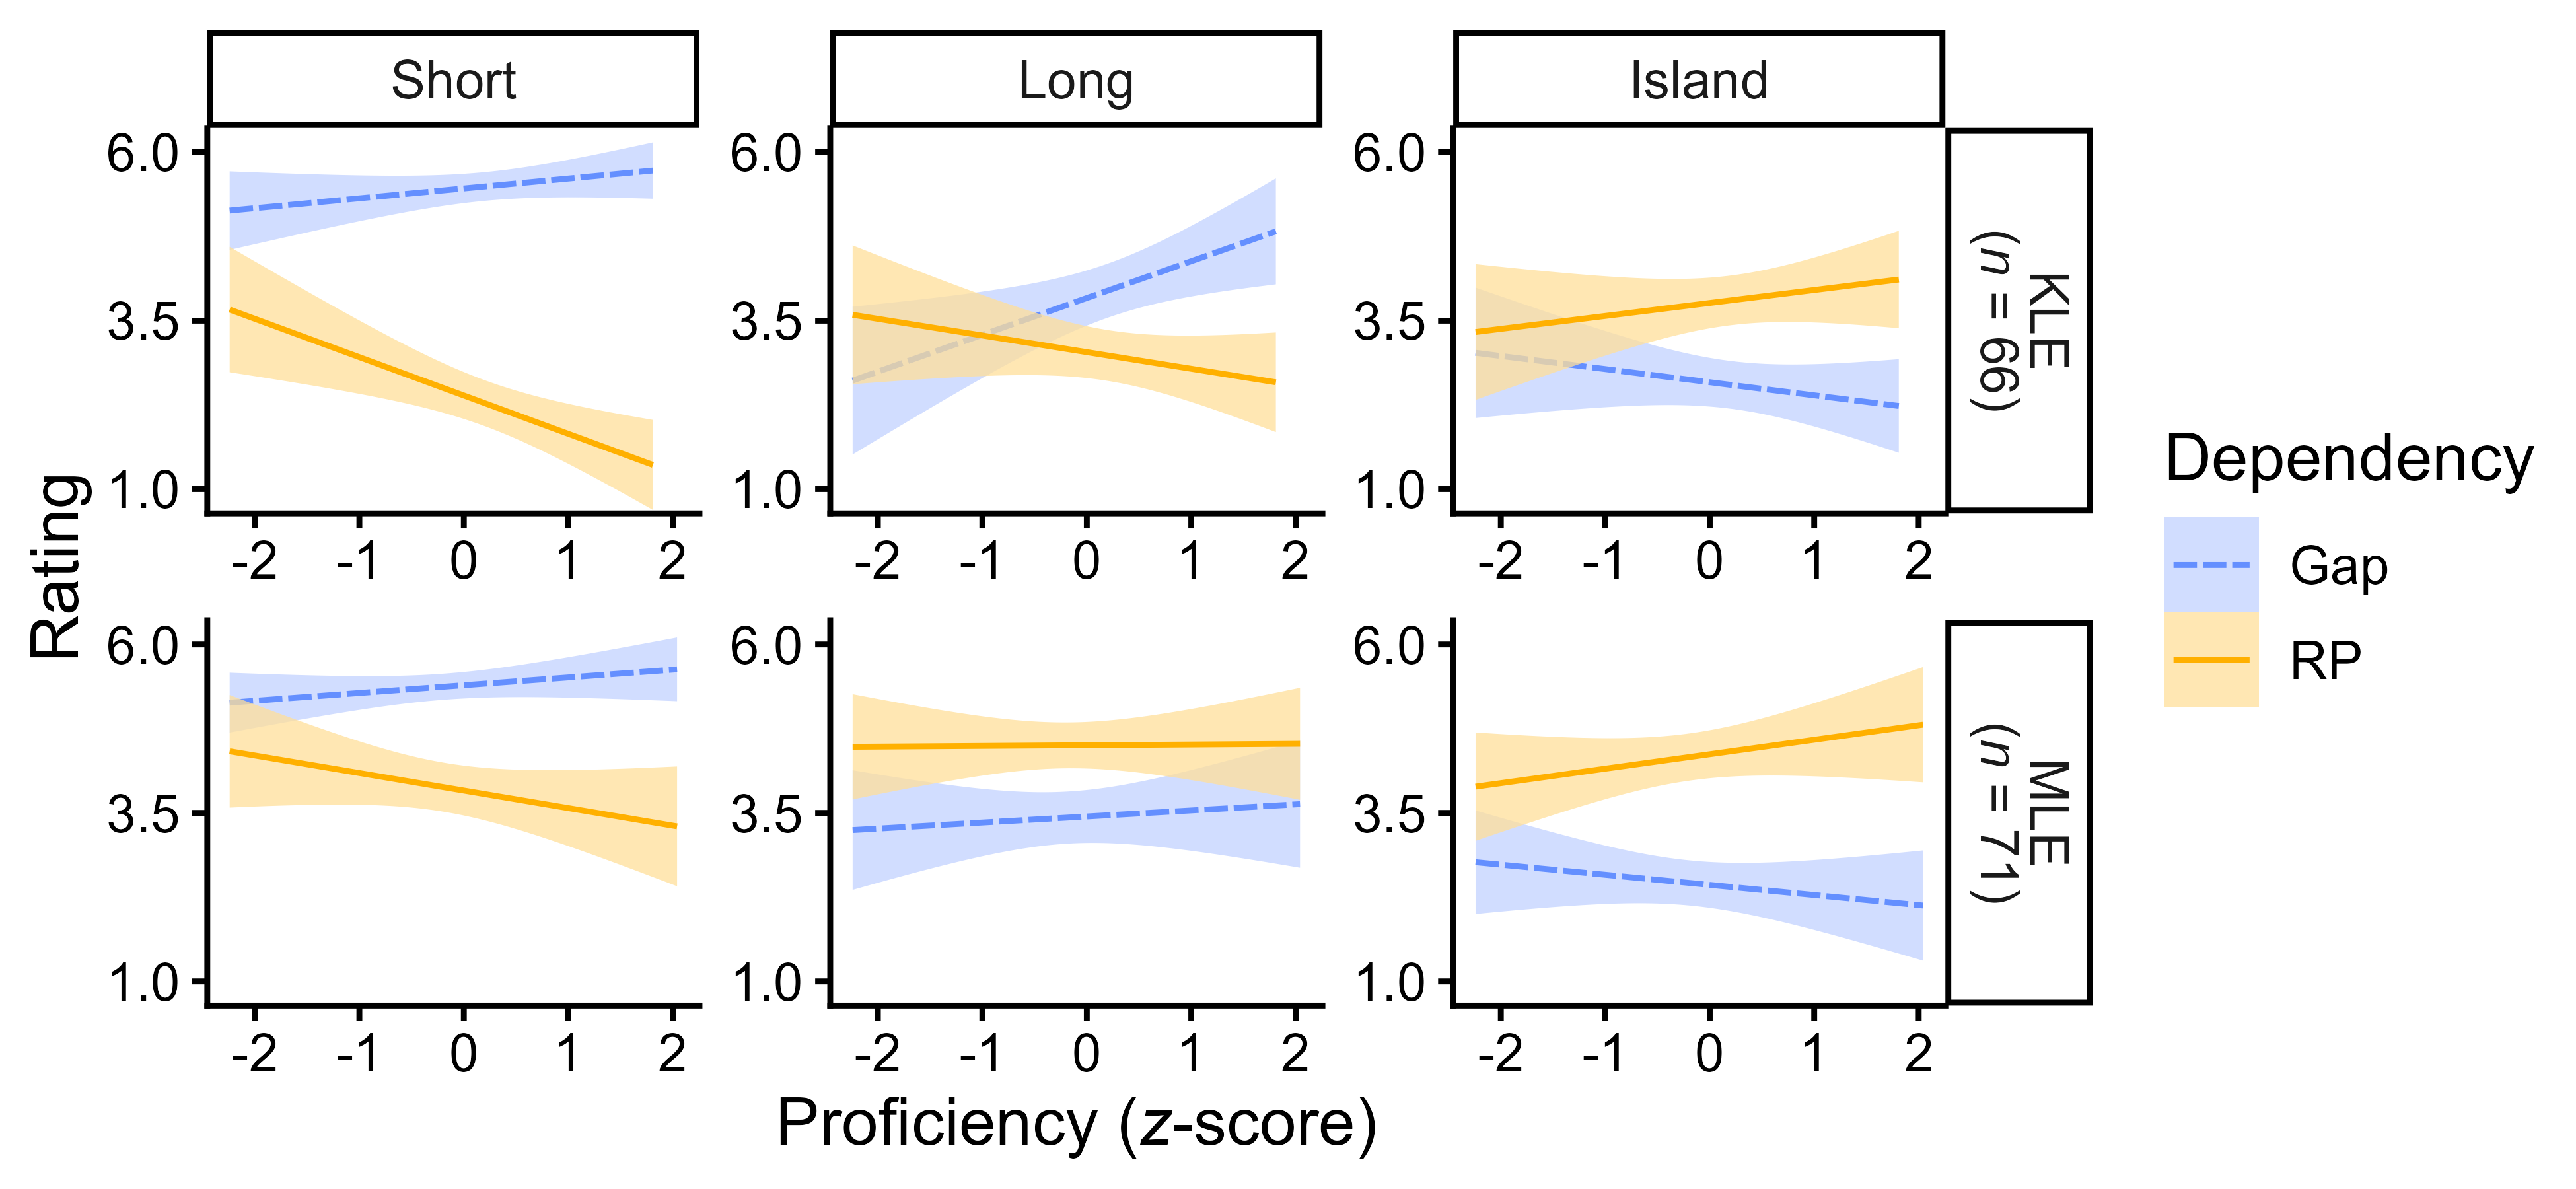
\includegraphics{../analysis/plots/src_ajt_rating_proficiency.png}
% \textit{Note}. Shading indicates 95\% \textit{CI}s.
% \vspace{-12pt}
% \end{figure}

% ORC Model
\DTLloaddb{dt-orc-ajt-rating-proficiency-model}{../analysis/tables/orc_ajt_rating_proficiency_model.csv}
\ExplSyntaxOn
\tl_clear:N \tblrbody
\tl_build_begin:N \tblrbody
\DTLforeach{dt-orc-ajt-rating-proficiency-model}{\coli=Parameter,\colii=Estimate,\coliii=$SE$,\coliv=$z$,\colv=$p$}{\tl_build_put_right:Ne \tblrbody {\exp_not:V \coli & \exp_not:V \colii & \exp_not:V \coliii & \exp_not:V \coliv & \exp_not:V \colv\\}}
\tl_build_end:N \tblrbody
\ExplSyntaxOff
\begin{longtblr}[caption={Summary of cumulative link mixed model for proficiency effects on ratings in the ORC acceptability judgment task}, label={tblr:app-orc-ajt-rating-proficiency-model}, expand=\tblrbody, remark{Note}={Model formula: Rating \~{} Dependency * Environment * Pairing * Proficiency + (1 + Dependency * Environment | Participant) + (0 + Dependency * Environment | Item); reference level: Gap + Short + KE; estimate unit: logit; intercept: grand mean.}]{colspec={lX[r]X[r]X[r]X[r]}}\toprule
Parameter & Estimate~($\hat{\beta}$) & \textit{SE} & $z$ & $p$\\\midrule
\tblrbody\bottomrule
\end{longtblr}
\vspace{-12pt}

% ORC Posthoc
\begin{table}
\caption{Post-hoc tests for L2 proficiency effects on ratings in the ORC acceptability judgment task}\label{tab:app-orc-ajt-rating-proficiency-posthoc}
\raggedright\setstretch{1}
\begin{tabularx}{\textwidth}{lXXYYYY}\toprule
Group & Environment & Contrast & Estimate~($\hat{\beta}$) & \textit{SE} & $z$ & $p$ \\\midrule
\csvreader[late after line=\\,late after last line=\\\bottomrule]
{../analysis/tables/orc_ajt_rating_proficiency_posthoc.csv}{}{\csvcoli & \csvcolii & \csvcoliii & \csvcoliv & \csvcolv & \csvcolvi & \csvcolvii}
\end{tabularx}
\textit{Note}. Adjustment to $p$-values done via multiple $t$ method for 6 tests.
\vspace{-12pt}
\end{table}

% SRC Model
\DTLloaddb{dt-src-ajt-rating-proficiency-model}{../analysis/tables/src_ajt_rating_proficiency_model.csv}
\ExplSyntaxOn
\tl_clear:N \tblrbody
\tl_build_begin:N \tblrbody
\DTLforeach{dt-src-ajt-rating-proficiency-model}{\coli=Parameter,\colii=Estimate,\coliii=$SE$,\coliv=$z$,\colv=$p$}{\tl_build_put_right:Ne \tblrbody {\exp_not:V \coli & \exp_not:V \colii & \exp_not:V \coliii & \exp_not:V \coliv & \exp_not:V \colv\\}}
\tl_build_end:N \tblrbody
\ExplSyntaxOff
\begin{longtblr}[caption={Summary of cumulative link mixed model for proficiency effects on ratings in the SRC acceptability judgment task}, label={tblr:app-src-ajt-rating-proficiency-model}, expand=\tblrbody, remark{Note}={Model formula: Rating \~{} Dependency * Environment * Pairing * Proficiency + (1 + Dependency * Environment | Participant) + (0 + Dependency * Environment | Item); reference level: Gap + Short + KE; estimate unit: logit; intercept: grand mean.}]{colspec={lX[r]X[r]X[r]X[r]}}\toprule
Parameter & Estimate~($\hat{\beta}$) & \textit{SE} & $z$ & $p$\\\midrule
\tblrbody\bottomrule
\end{longtblr}
\vspace{-12pt}

% SRC Posthoc
\begin{table}
\caption{Post-hoc tests for L2 proficiency effects on ratings in the SRC acceptability judgment task}\label{tab:app-src-ajt-rating-proficiency-posthoc}
\raggedright\setstretch{1}
\begin{tabularx}{\textwidth}{lXXYYYY}\toprule
Group & Environment & Contrast & Estimate~($\hat{\beta}$) & \textit{SE} & $z$ & $p$ \\\midrule
\csvreader[late after line=\\,late after last line=\\\bottomrule]
{../analysis/tables/src_ajt_rating_proficiency_posthoc.csv}{}{\csvcoli & \csvcolii & \csvcoliii & \csvcoliv & \csvcolv & \csvcolvi & \csvcolvii}
\end{tabularx}
\textit{Note}. Adjustment to $p$-values done via multiple $t$ method for 6 tests.
\end{table}

%========================================================%
\section{By-participant rating patterns}\label{app-ajt-individual}
%========================================================%

% ORC Proportions
% \DTLloaddb{dt-ajt-acceptor}{../analysis/tables/ajt_acceptor.csv}
% \ExplSyntaxOn
% \tl_clear:N \tblrbody
% \tl_build_begin:N \tblrbody
% \DTLforeach[\equal{\study}{ORC}]{dt-ajt-acceptor}{\study=study,\coli=Pairing,\colii=Environment,\coliii=Type,\coliv=Count,\colv=Percent}{\tl_build_put_right:Ne \tblrbody {\exp_not:V \coli & \exp_not:V \colii & \exp_not:V \coliii & \exp_not:V \coliv & \exp_not:V \colv\\}}
% \tl_build_end:N \tblrbody
% \ExplSyntaxOff
% \begin{longtblr}[caption={Percentage of RP acceptors, RP rejectors, and inconsistent raters by environment in the ORC acceptability judgment task}, label={tblr:app-orc-ajt-acceptor}, expand=\tblrbody, remark{Note} = {EE~= ENS in English; KE~= KLE in English; ME~= MLE in English; KK~= KLE in Korean; MM~= MLE in Mandarin.}]{colspec={XXXX[r]X[r]}}\toprule
% Pairing & Environment & Type & Count & \%\\\midrule
% \tblrbody\bottomrule
% \end{longtblr}
% \vspace{-12pt}

% SRC Proportions
% \ExplSyntaxOn
% \tl_clear:N \tblrbody
% \tl_build_begin:N \tblrbody
% \DTLforeach[\equal{\study}{SRC}]{dt-ajt-acceptor}{\study=study,\coli=Pairing,\colii=Environment,\coliii=Type,\coliv=Count,\colv=Percent}{\tl_build_put_right:Ne \tblrbody {\exp_not:V \coli & \exp_not:V \colii & \exp_not:V \coliii & \exp_not:V \coliv & \exp_not:V \colv\\}}
% \tl_build_end:N \tblrbody
% \ExplSyntaxOff
% \begin{longtblr}[caption={Percentage of RP acceptors, RP rejectors, and inconsistent raters by environment in the SRC acceptability judgment task}, label={tblr:app-src-ajt-acceptor}, expand=\tblrbody, remark{Note} = {EE~= ENS in English; KE~= KLE in English; ME~= MLE in English; KK~= KLE in Korean; MM~= MLE in Mandarin.}]{colspec={XXXX[r]X[r]}}\toprule
% Pairing & Environment & Type & Count & \%\\\midrule
% \tblrbody\bottomrule
% \end{longtblr}
% \vspace{-12pt}

% ORC Figure
% \begin{figure}
% \caption{Percentage of RP acceptors, RP rejectors, and inconsistent raters by environment in the ORC acceptability judgment tasks} \label{fig:app-ajt-acceptor-orc}
% \raggedright\setstretch{1}
% 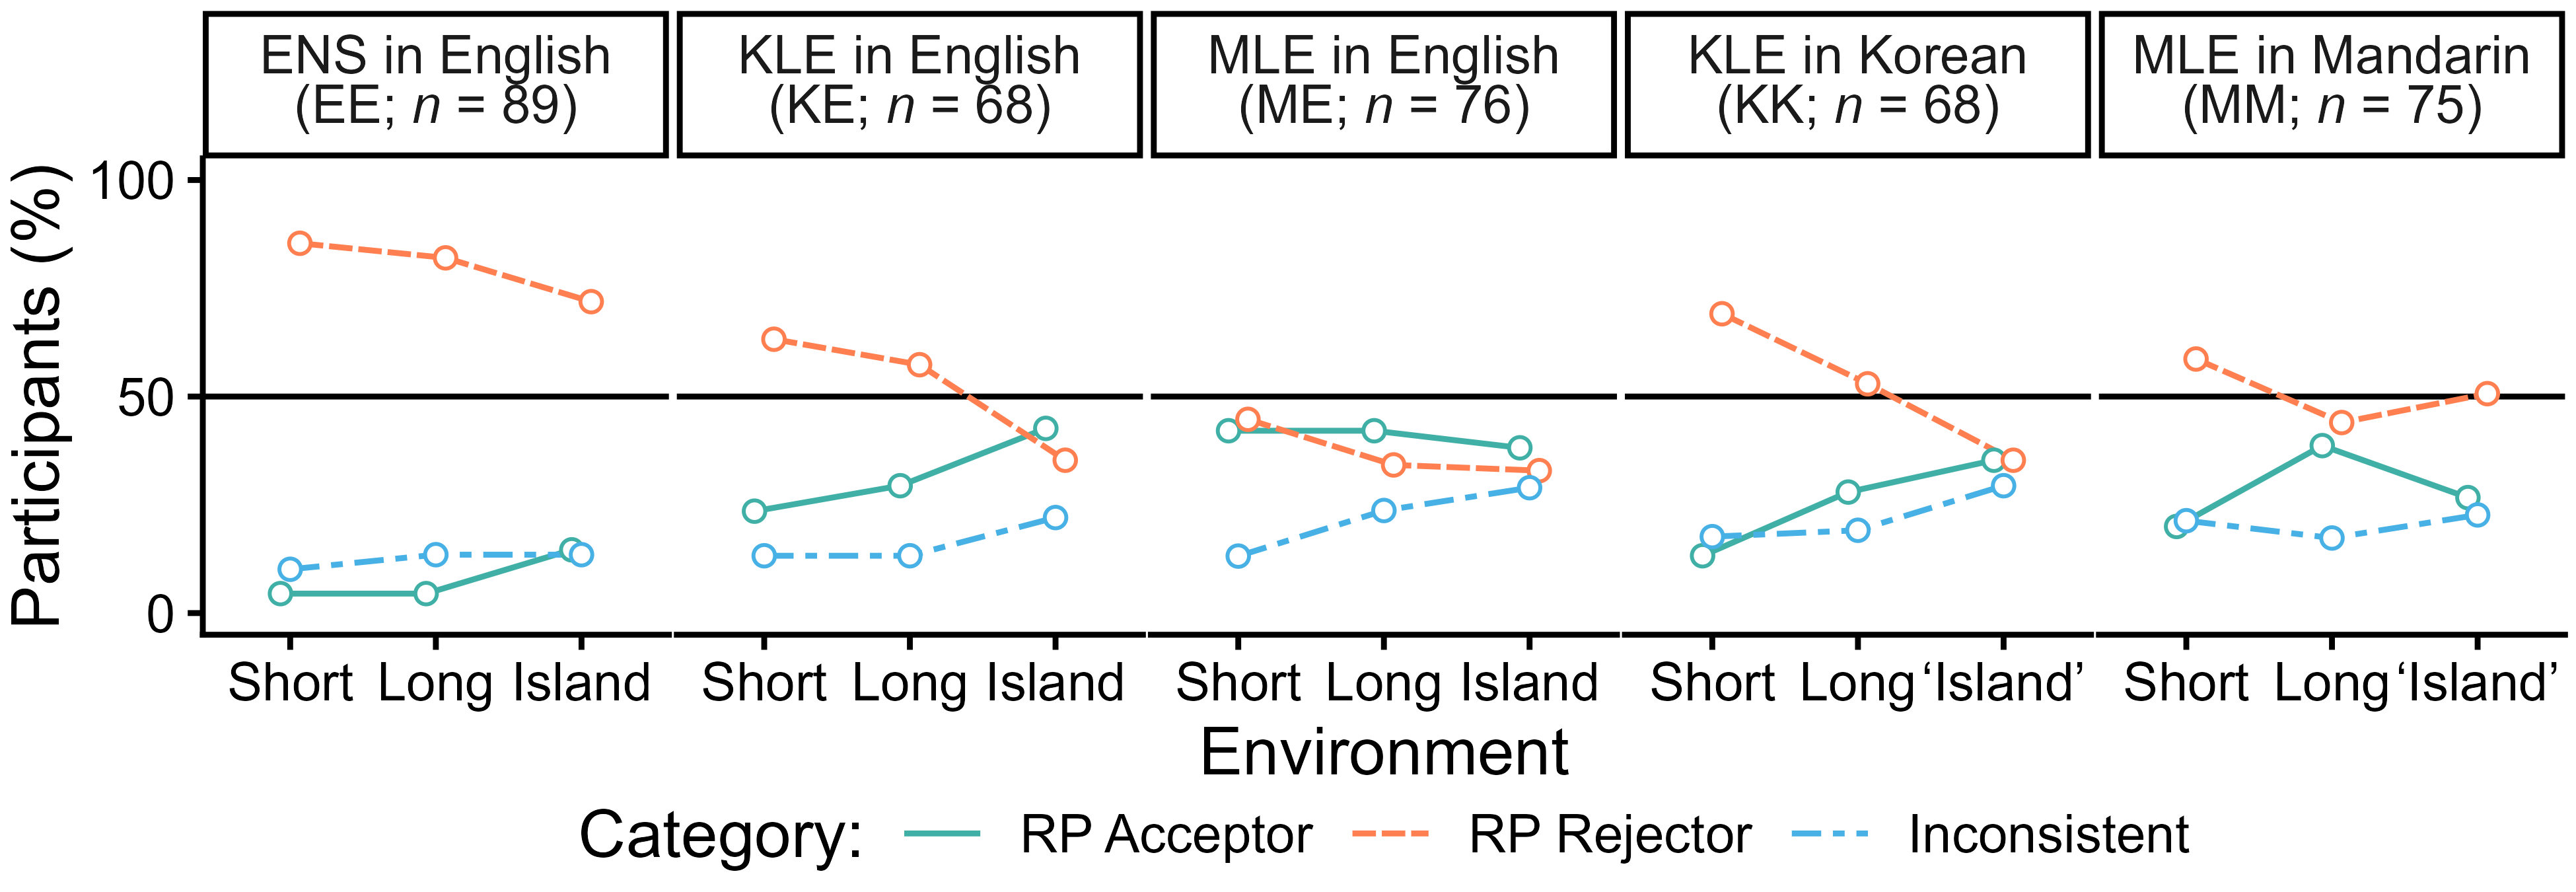
\includegraphics[width=\textwidth]{../analysis/plots/orc_ajt_acceptor.png}
% \vspace{-12pt}
% \end{figure}

% SRC Figure
% \begin{figure}
% \caption{Percentage of RP acceptors, RP rejectors, and inconsistent raters by environment in the SRC acceptability judgment tasks} \label{fig:app-ajt-acceptor-src}
% \raggedright\setstretch{1}
% 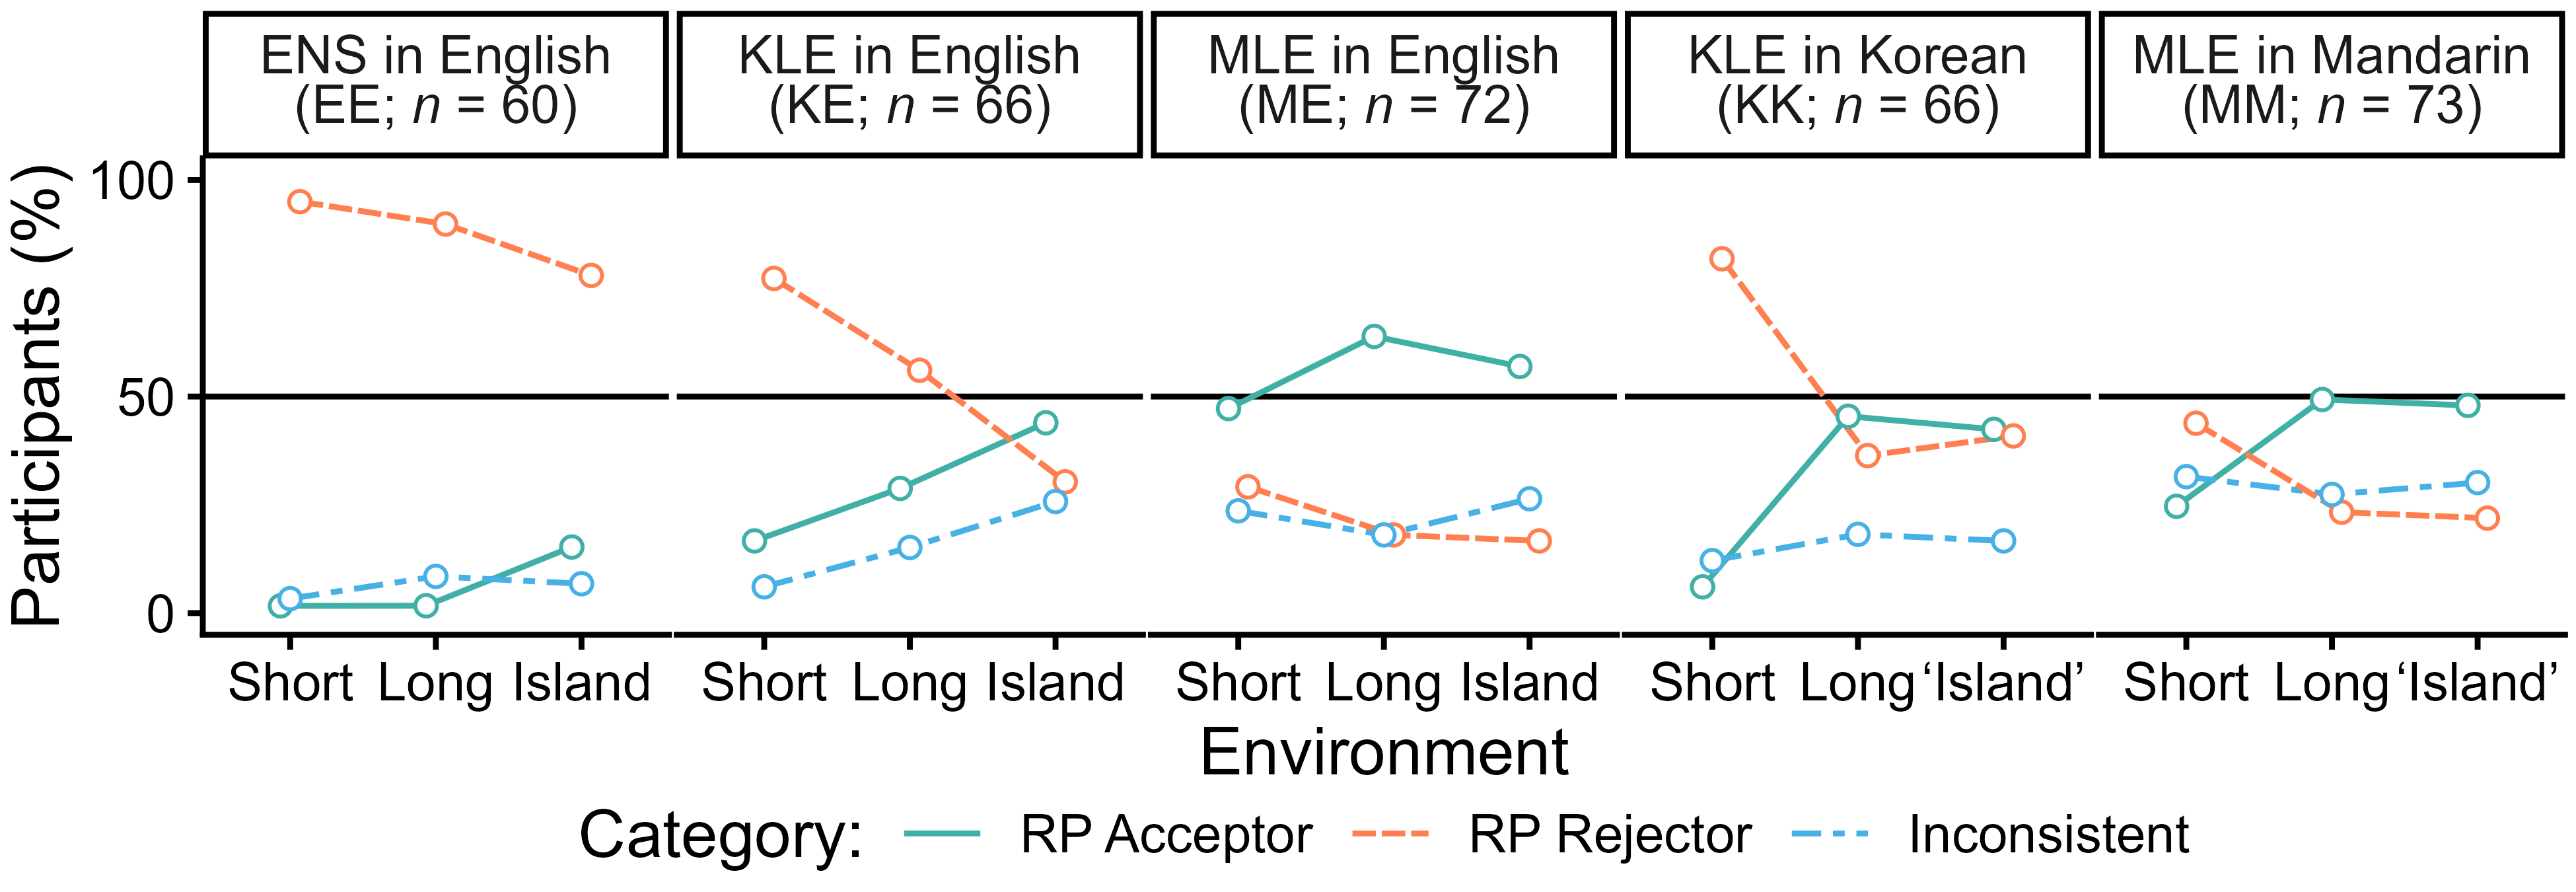
\includegraphics[width=\textwidth]{../analysis/plots/src_ajt_acceptor.png}
% \vspace{-12pt}
% \end{figure}

% ORC Model
\DTLloaddb{dt-orc-ajt-acceptor-model}{../analysis/tables/orc_ajt_acceptor_model.csv}
\ExplSyntaxOn
\tl_clear:N \tblrbody
\tl_build_begin:N \tblrbody
\DTLforeach{dt-orc-ajt-acceptor-model}{\coli=Parameter,\colii=Estimate,\coliii=$SE$,\coliv=$z$,\colv=$p$}{\tl_build_put_right:Ne \tblrbody {\exp_not:V \coli & \exp_not:V \colii & \exp_not:V \coliii & \exp_not:V \coliv & \exp_not:V \colv\\}}
\tl_build_end:N \tblrbody
\ExplSyntaxOff
\begin{longtblr}[caption={Summary of mixed-effects logistic regression model for RP acceptors in the ORC acceptability judgment task}, label={tblr:app-orc-ajt-acceptor-model}, expand=\tblrbody, remark{Note}={Model formula: Acceptor \~{} Environment * Pairing + (1 | Participant); reference level: Short + EE; estimate unit: logit; intercept: grand mean.}]{colspec={lX[r]X[r]X[r]X[r]}}\toprule
Parameter & Estimate~($\hat{\beta}$) & \textit{SE} & $z$ & $p$\\\midrule
\tblrbody\bottomrule
\end{longtblr}
\vspace{-12pt}

% ORC Posthoc
\begin{table}
\caption{Post-hoc tests for RP acceptors in the ORC acceptability judgment task}\label{tab:app-orc-ajt-acceptor-posthoc}
\raggedright\setstretch{1}
\begin{tabularx}{\textwidth}{lXXYYYY}\toprule
Pairing & Contrast & Estimate~($\hat{\beta}$) & \textit{SE} & $z$ & $p$ \\\midrule
\csvreader[late after line=\\,late after last line=\\\bottomrule]
{../analysis/tables/orc_ajt_acceptor_posthoc.csv}{}{\csvcoli & \csvcolii & \csvcoliii & \csvcoliv & \csvcolv & \csvcolvi}
\end{tabularx}
\textit{Note}. Adjustment to $p$-values done via multiple $t$ method for 15 tests.
\vspace{-12pt}
\end{table}

% SRC Model
\DTLloaddb{dt-src-ajt-acceptor-model}{../analysis/tables/src_ajt_acceptor_model.csv}
\ExplSyntaxOn
\tl_clear:N \tblrbody
\tl_build_begin:N \tblrbody
\DTLforeach{dt-src-ajt-acceptor-model}{\coli=Parameter,\colii=Estimate,\coliii=$SE$,\coliv=$z$,\colv=$p$}{\tl_build_put_right:Ne \tblrbody {\exp_not:V \coli & \exp_not:V \colii & \exp_not:V \coliii & \exp_not:V \coliv & \exp_not:V \colv\\}}
\tl_build_end:N \tblrbody
\ExplSyntaxOff
\begin{longtblr}[caption={Summary of mixed-effects logistic regression model for RP acceptors in the SRC acceptability judgment task}, label={tblr:app-src-ajt-acceptor-model}, expand=\tblrbody, remark{Note}={Model formula: Acceptor \~{} Environment * Pairing + (1 | Participant); reference level: Short + EE; estimate unit: logit; intercept: grand mean.}]{colspec={lX[r]X[r]X[r]X[r]}}\toprule
Parameter & Estimate~($\hat{\beta}$) & \textit{SE} & $z$ & $p$\\\midrule
\tblrbody\bottomrule
\end{longtblr}
\vspace{-12pt}

% SRC Posthoc
\begin{table}
\caption{Post-hoc tests for RP acceptors in the SRC acceptability judgment task}\label{tab:app-src-ajt-acceptor-posthoc}
\raggedright\setstretch{1}
\begin{tabularx}{\textwidth}{lXXYYYY}\toprule
Pairing & Contrast & Estimate~($\hat{\beta}$) & \textit{SE} & $z$ & $p$ \\\midrule
\csvreader[late after line=\\,late after last line=\\\bottomrule]
{../analysis/tables/src_ajt_acceptor_posthoc.csv}{}{\csvcoli & \csvcolii & \csvcoliii & \csvcoliv & \csvcolv & \csvcolvi}
\end{tabularx}
\textit{Note}. Adjustment to $p$-values done via multiple $t$ method for 15 tests.
\vspace{-12pt}
\end{table}

%========================================================%
\section{L2 proficiency effects for by-participant rating patterns}\label{app-ajt-individual-proficiency}
%========================================================%

% ORC Means
% \DTLloaddb{dt-ajt-acceptor_proficiency2}{../analysis/tables/ajt_acceptor_environment_proficiency2.csv}
% \ExplSyntaxOn
% \tl_clear:N \tblrbody
% \tl_build_begin:N \tblrbody
% \DTLforeach[\equal{\study}{ORC}]{dt-ajt-acceptor_proficiency2}{\study=study,\coli=Group,\colii=Environment,\coliii=Mean,\coliv=$CI$}{\tl_build_put_right:Ne \tblrbody {\exp_not:V \coli & \exp_not:V \colii & \exp_not:V \coliii & \exp_not:V \coliv\\}}
% \tl_build_end:N \tblrbody
% \ExplSyntaxOff
% \begin{longtblr}[caption={Mean L2 proficiency for RP acceptors, RP rejectors, and inconsistent raters in the ORC acceptability judgment task}, label={tblr:app-orc-ajt-acceptor-proficiency}, expand=\tblrbody]{colspec={XXX[r]X[r]}}\toprule
% Group & Environment & Mean & 95\% \textit{CI} \\\midrule
% \tblrbody\bottomrule
% \end{longtblr}
% \vspace{-12pt}

% SRC Means
% \ExplSyntaxOn
% \tl_clear:N \tblrbody
% \tl_build_begin:N \tblrbody
% \DTLforeach[\equal{\study}{SRC}]{dt-ajt-acceptor_proficiency2}{\study=study,\coli=Group,\colii=Environment,\coliii=Mean,\coliv=$CI$}{\tl_build_put_right:Ne \tblrbody {\exp_not:V \coli & \exp_not:V \colii & \exp_not:V \coliii & \exp_not:V \coliv\\}}
% \tl_build_end:N \tblrbody
% \ExplSyntaxOff
% \begin{longtblr}[caption={Mean L2 proficiency for RP acceptors, RP rejectors, and inconsistent raters in the SRC acceptability judgment task}, label={tblr:app-src-ajt-acceptor-proficiency}, expand=\tblrbody]{colspec={XXX[r]X[r]}}\toprule
% Group & Environment & Mean & 95\% \textit{CI} \\\midrule
% \tblrbody\bottomrule
% \end{longtblr}
% \vspace{-12pt}

% ORC Figure
% \begin{figure}
% \caption{L2 proficiency scores for RP acceptors, RP rejectors, and inconsistent raters in the ORC English acceptability judgment task} \label{fig:app-ajt-acceptor-proficiency-orc}
% \raggedright\setstretch{1}
% 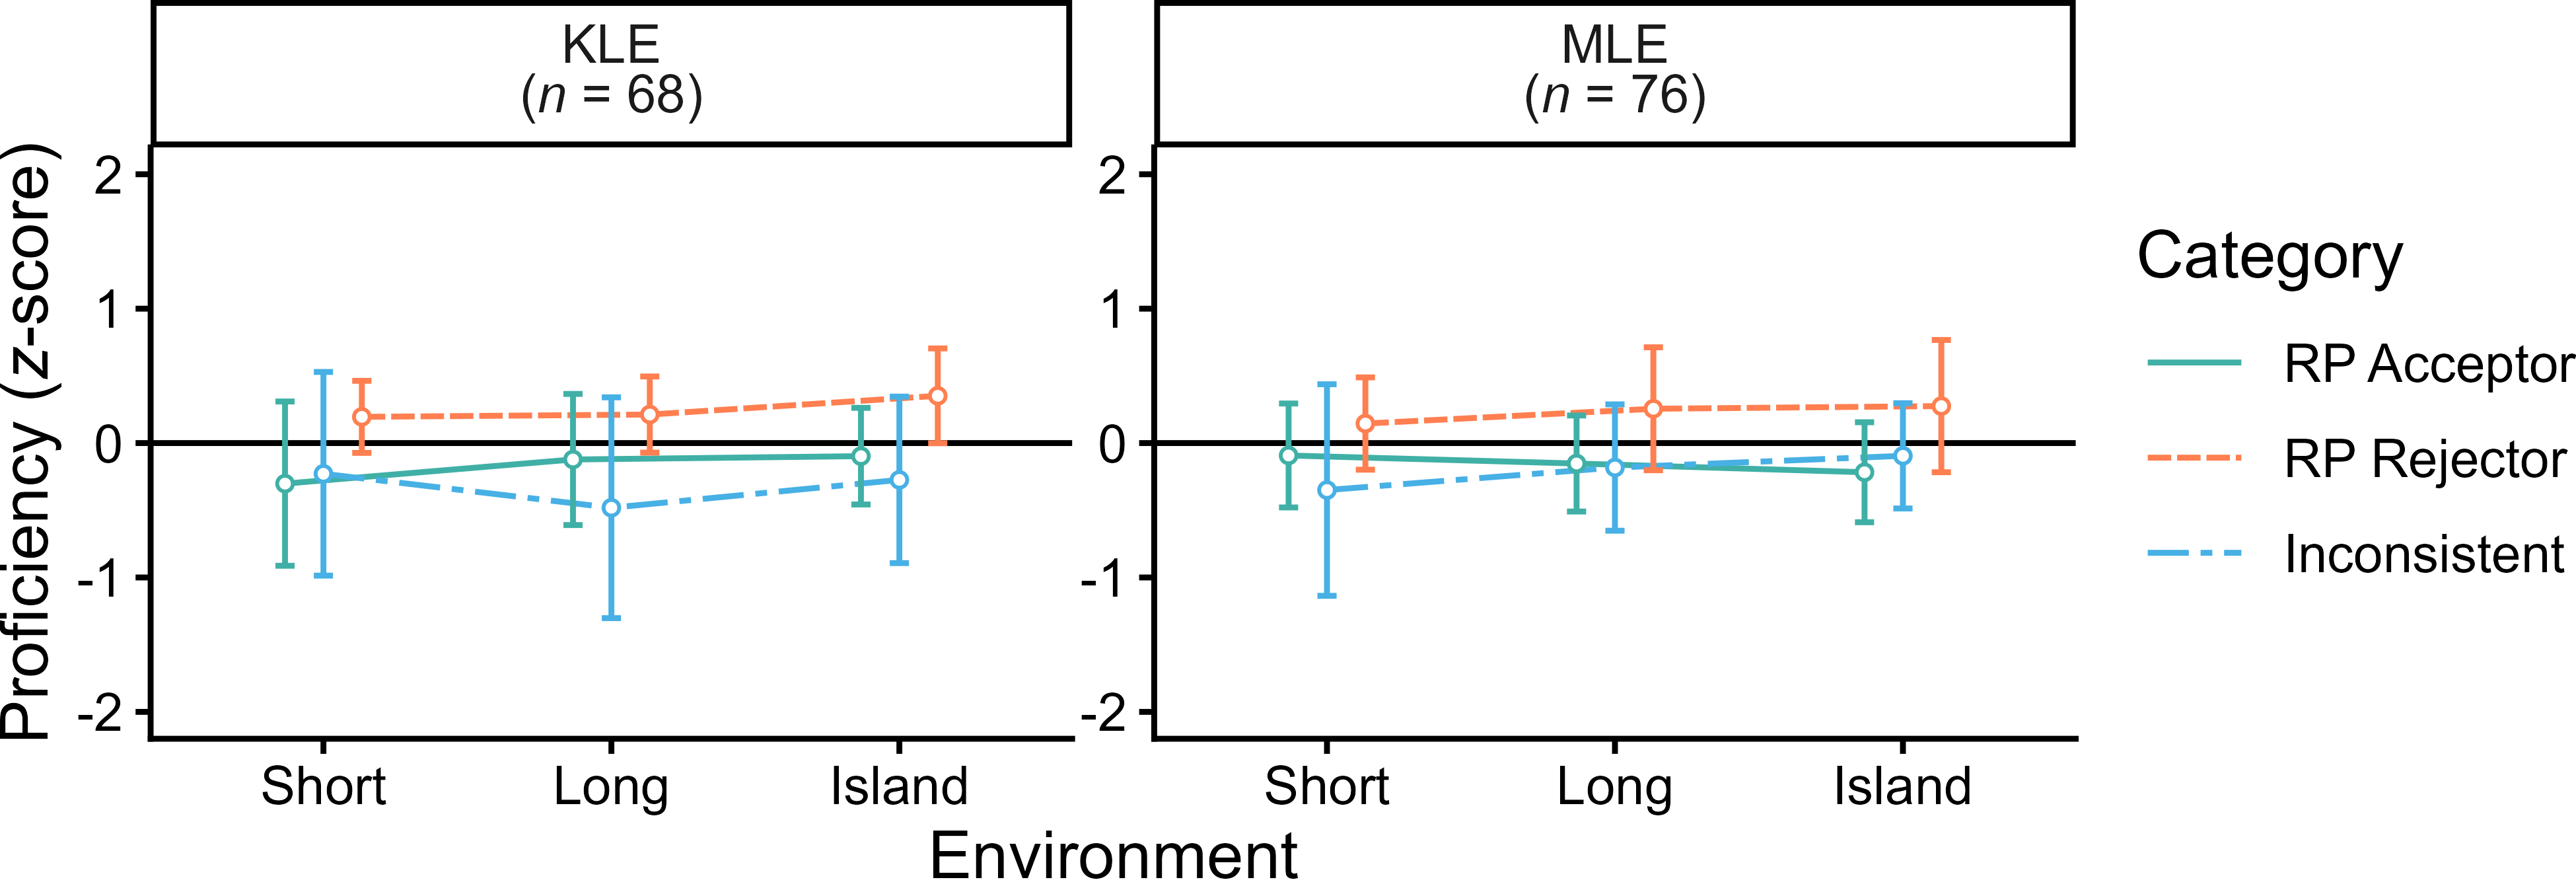
\includegraphics[width=\textwidth]{../analysis/plots/orc_ajt_acceptor_environment_proficiency2.png}
% \vspace{-12pt}
% \end{figure}

% SRC Figure
% \begin{figure}
% \caption{L2 proficiency scores for RP acceptors, RP rejectors, and inconsistent raters in the SRC English acceptability judgment task} \label{fig:app-ajt-acceptor-proficiency-src}
% \raggedright\setstretch{1}
% 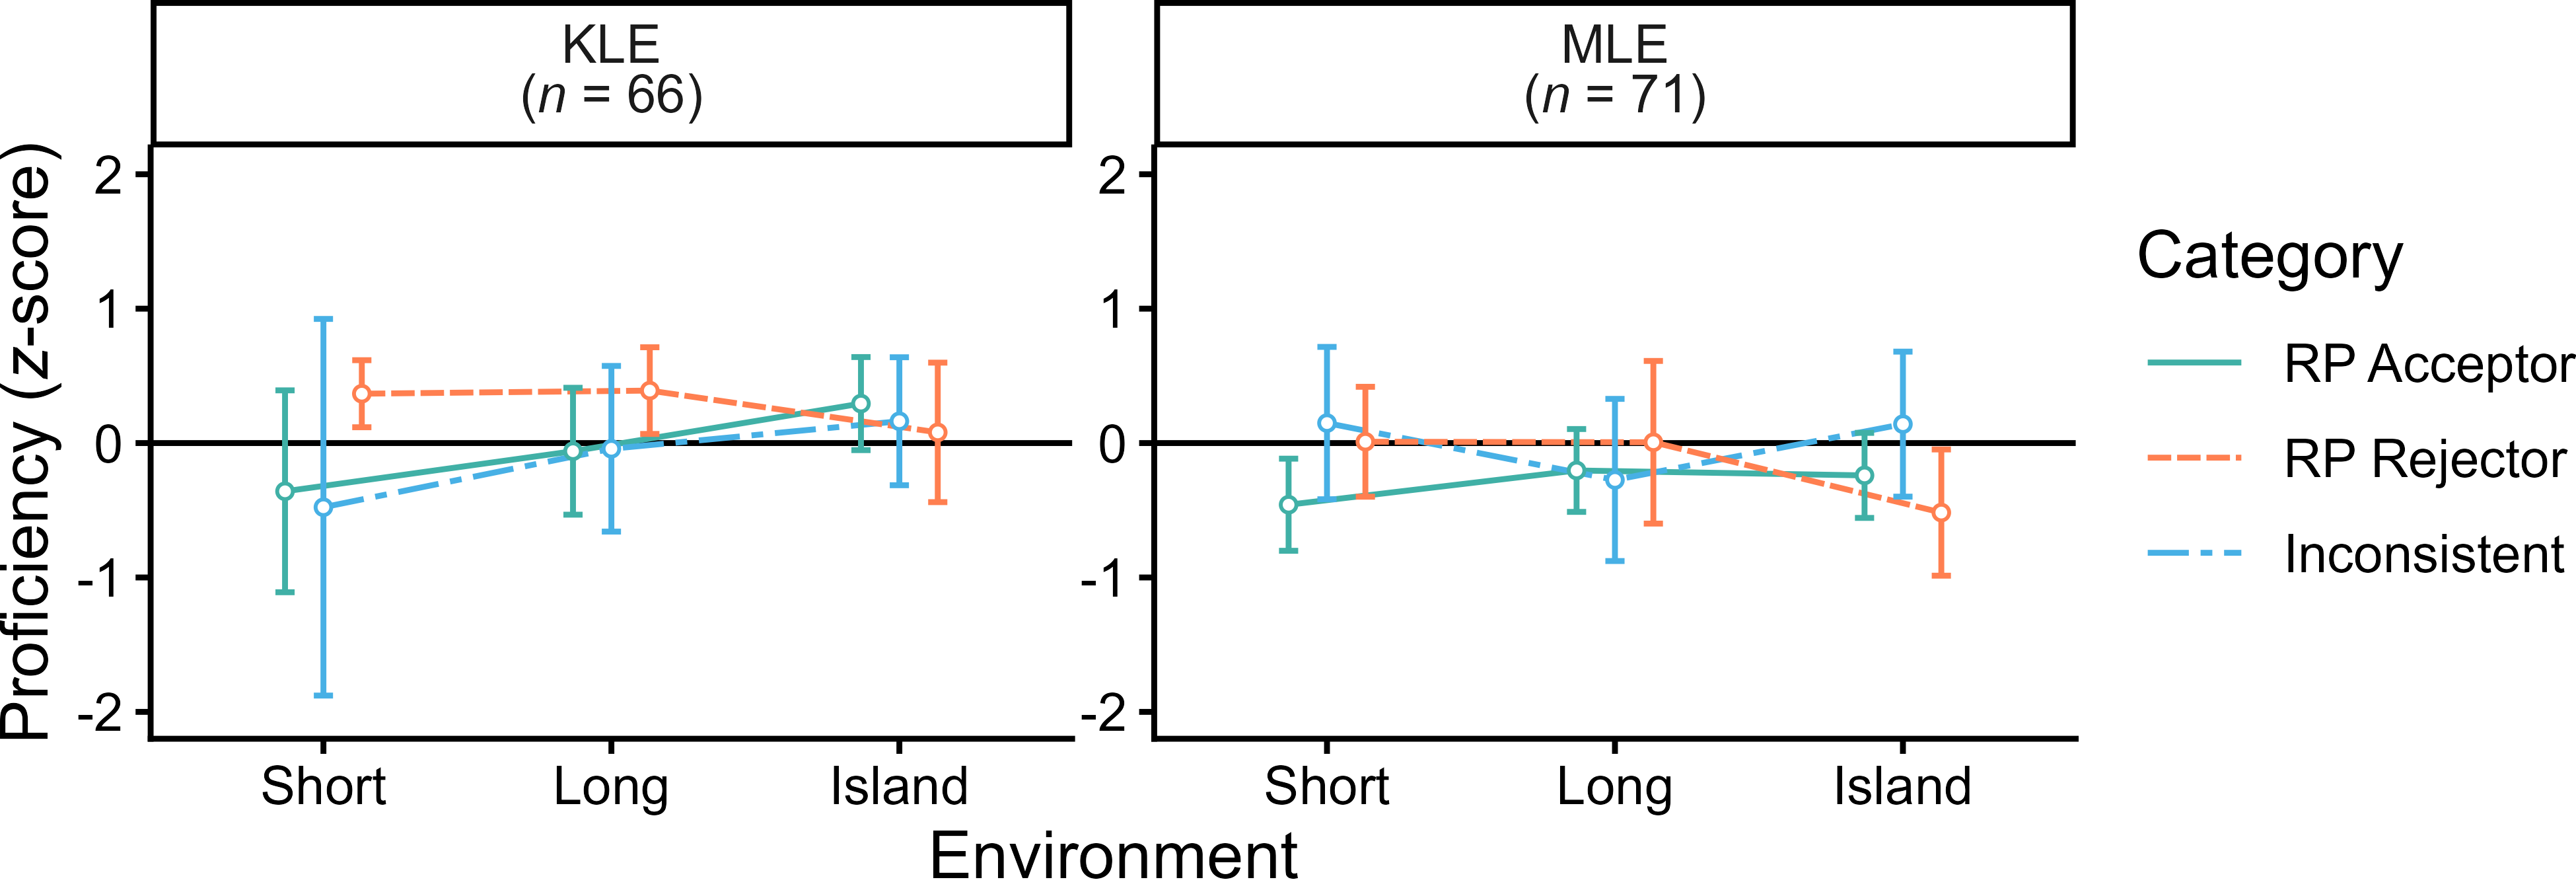
\includegraphics[width=\textwidth]{../analysis/plots/src_ajt_acceptor_environment_proficiency2.png}
% \vspace{-12pt}
% \end{figure}

% ORC Model
\DTLloaddb{dt-orc-ajt-acceptor-proficiency-model}{../analysis/tables/orc_ajt_acceptor_proficiency_model.csv}
\ExplSyntaxOn
\tl_clear:N \tblrbody
\tl_build_begin:N \tblrbody
\DTLforeach{dt-orc-ajt-acceptor-proficiency-model}{\coli=Parameter,\colii=Estimate,\coliii=$SE$,\coliv=$z$,\colv=$p$}{\tl_build_put_right:Ne \tblrbody {\exp_not:V \coli & \exp_not:V \colii & \exp_not:V \coliii & \exp_not:V \coliv & \exp_not:V \colv\\}}
\tl_build_end:N \tblrbody
\ExplSyntaxOff
\begin{longtblr}[caption={Summary of mixed-effects logistic regression model for L2 proficiency effects on RP acceptors in the ORC acceptability judgment task}, label={tblr:app-orc-ajt-acceptor-proficiency-model}, expand=\tblrbody, remark{Note}={Model formula: Acceptor \~{} Environment * Group * Proficiency + (1 | Participant); reference level: Short + KE; estimate unit: logit; intercept: grand mean.}]{colspec={lX[r]X[r]X[r]X[r]}}\toprule
Parameter & Estimate~($\hat{\beta}$) & \textit{SE} & $z$ & $p$\\\midrule
\tblrbody\bottomrule
\end{longtblr}
\vspace{-12pt}

% ORC Posthoc
\begin{table}
\caption{Post-hoc tests for L2 proficiency trend on RP acceptors in the ORC acceptability judgment task}\label{tab:app-orc-ajt-acceptor-proficiency-posthoc}
\raggedright\setstretch{1}
\begin{tabularx}{\textwidth}{XXYYYY}\toprule
Group & Environment & Estimate~($\hat{\beta}$) & \textit{SE} & $z$ & $p$ \\\midrule
\csvreader[late after line=\\,late after last line=\\\bottomrule]
{../analysis/tables/orc_ajt_acceptor_proficiency_posthoc.csv}{}{\csvcoli & \csvcolii & \csvcoliii & \csvcoliv & \csvcolv & \csvcolvi}
\end{tabularx}
\textit{Note}. Adjustment to $p$-values done via multiple $t$ method for 6 tests.
\vspace{-12pt}
\end{table}

% SRC Model
\DTLloaddb{dt-src-ajt-acceptor-proficiency-model}{../analysis/tables/src_ajt_acceptor_proficiency_model.csv}
\ExplSyntaxOn
\tl_clear:N \tblrbody
\tl_build_begin:N \tblrbody
\DTLforeach{dt-src-ajt-acceptor-proficiency-model}{\coli=Parameter,\colii=Estimate,\coliii=$SE$,\coliv=$z$,\colv=$p$}{\tl_build_put_right:Ne \tblrbody {\exp_not:V \coli & \exp_not:V \colii & \exp_not:V \coliii & \exp_not:V \coliv & \exp_not:V \colv\\}}
\tl_build_end:N \tblrbody
\ExplSyntaxOff
\begin{longtblr}[caption={Summary of mixed-effects logistic regression model for L2 proficiency effects on RP acceptors in the SRC acceptability judgment task}, label={tblr:app-src-ajt-acceptor-proficiency-model}, expand=\tblrbody, remark{Note}={Model formula: Acceptor \~{} Environment * Group * Proficiency + (1 | Participant); reference level: Short + KE; estimate unit: logit; intercept: grand mean.}]{colspec={lX[r]X[r]X[r]X[r]}}\toprule
Parameter & Estimate~($\hat{\beta}$) & \textit{SE} & $z$ & $p$\\\midrule
\tblrbody\bottomrule
\end{longtblr}
\vspace{-12pt}

% SRC Posthoc
\begin{table}
\caption{Post-hoc tests for L2 proficiency trend on RP acceptors in the SRC acceptability judgment task}\label{tab:app-src-ajt-acceptor-proficiency-posthoc}
\raggedright\setstretch{1}
\begin{tabularx}{\textwidth}{XXYYYY}\toprule
Group & Environment & Estimate~($\hat{\beta}$) & \textit{SE} & $z$ & $p$ \\\midrule
\csvreader[late after line=\\,late after last line=\\\bottomrule]
{../analysis/tables/src_ajt_acceptor_proficiency_posthoc.csv}{}{\csvcoli & \csvcolii & \csvcoliii & \csvcoliv & \csvcolv & \csvcolvi}
\end{tabularx}
\textit{Note}. Adjustment to $p$-values done via multiple $t$ method for 6 tests.
\vspace{-12pt}
\end{table}

%========================================================%
% \section{Transfer effects}\label{app-ajt-transfer}
%========================================================%

% ORC Figure
% \begin{figure}
% \caption{Percentage of RP acceptors by category in the English ORC acceptability judgment task} \label{fig:app-orc-ajt-acceptor-type}
% \raggedright\setstretch{1}
% 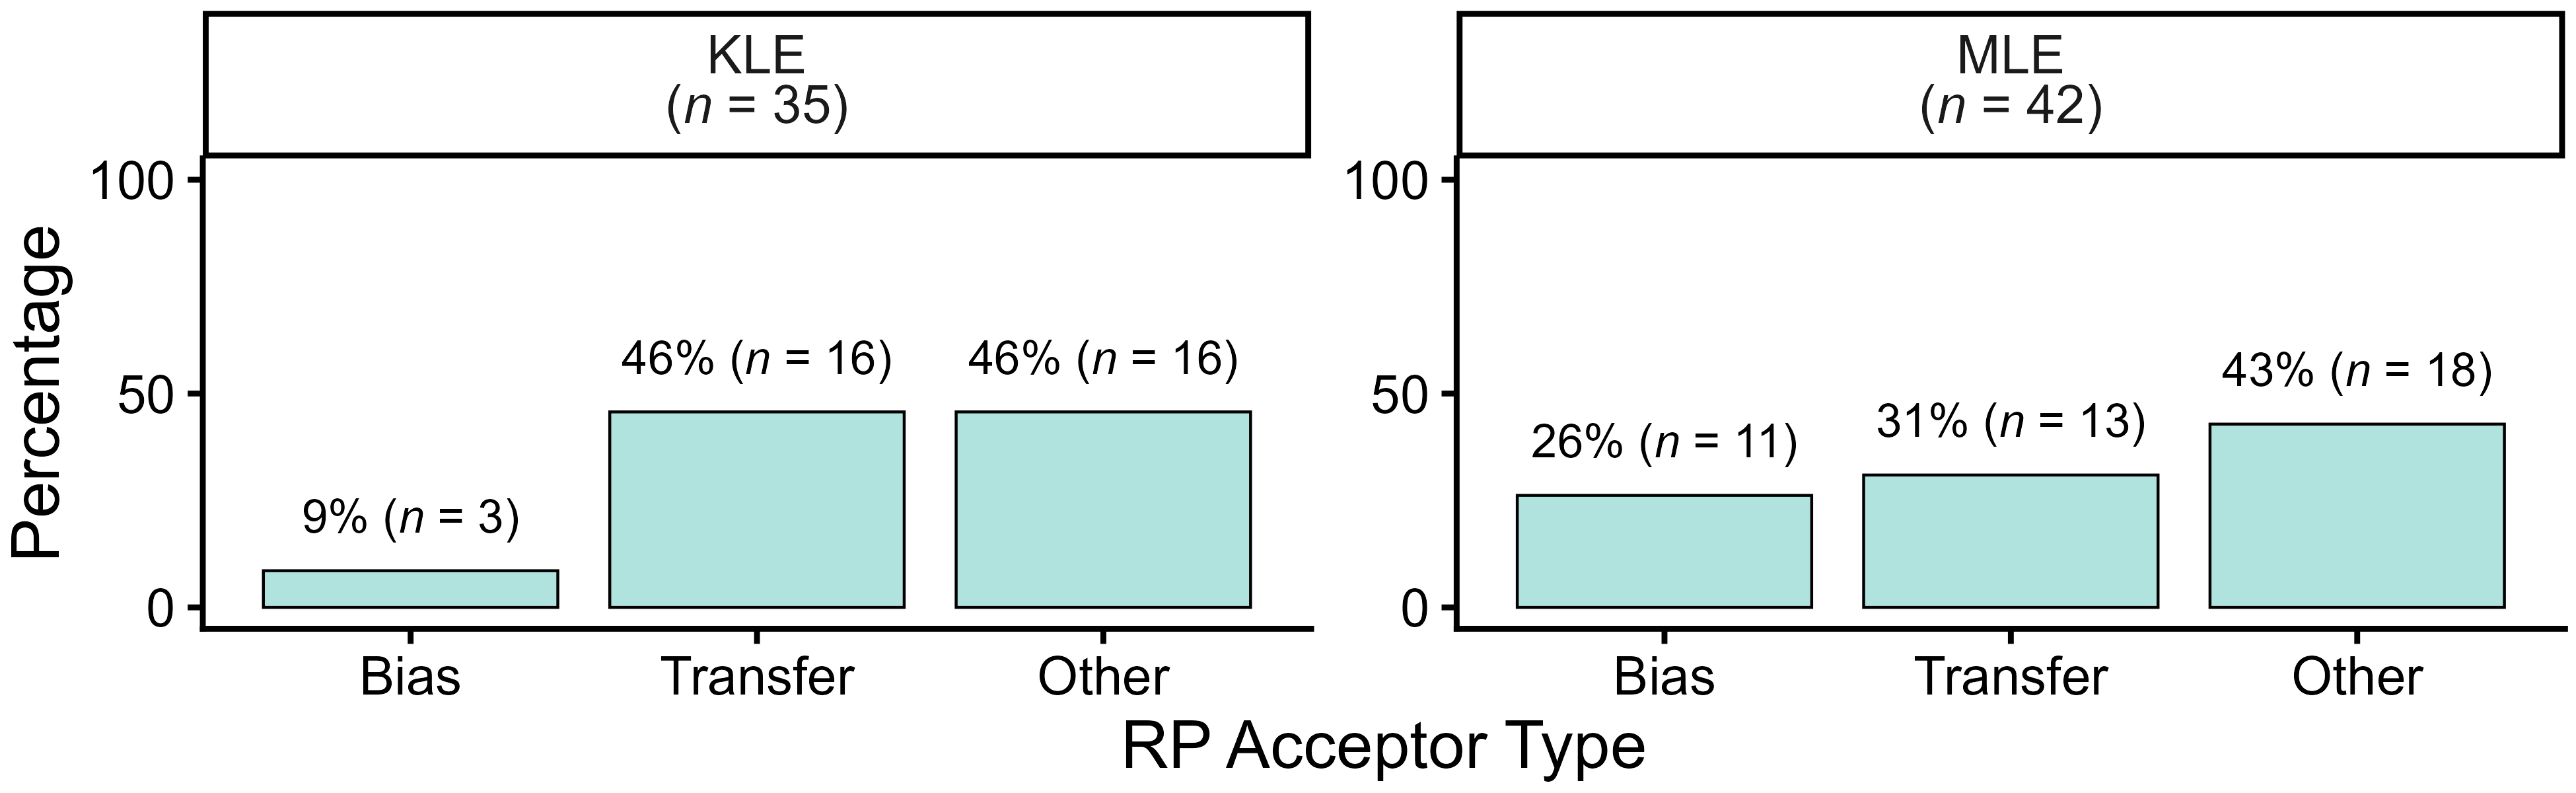
\includegraphics{../analysis/plots/orc_ajt_acceptor_type.png}
% \textit{Note}. Values are participant counts with percentages shown in parentheses.
% \vspace{-12pt}
% \end{figure}

% SRC Figure
% \begin{figure}
% \caption{Percentage of RP acceptors by category in the English SRC acceptability judgment task} \label{fig:app-src-ajt-acceptor-type}
% \raggedright\setstretch{1}
% 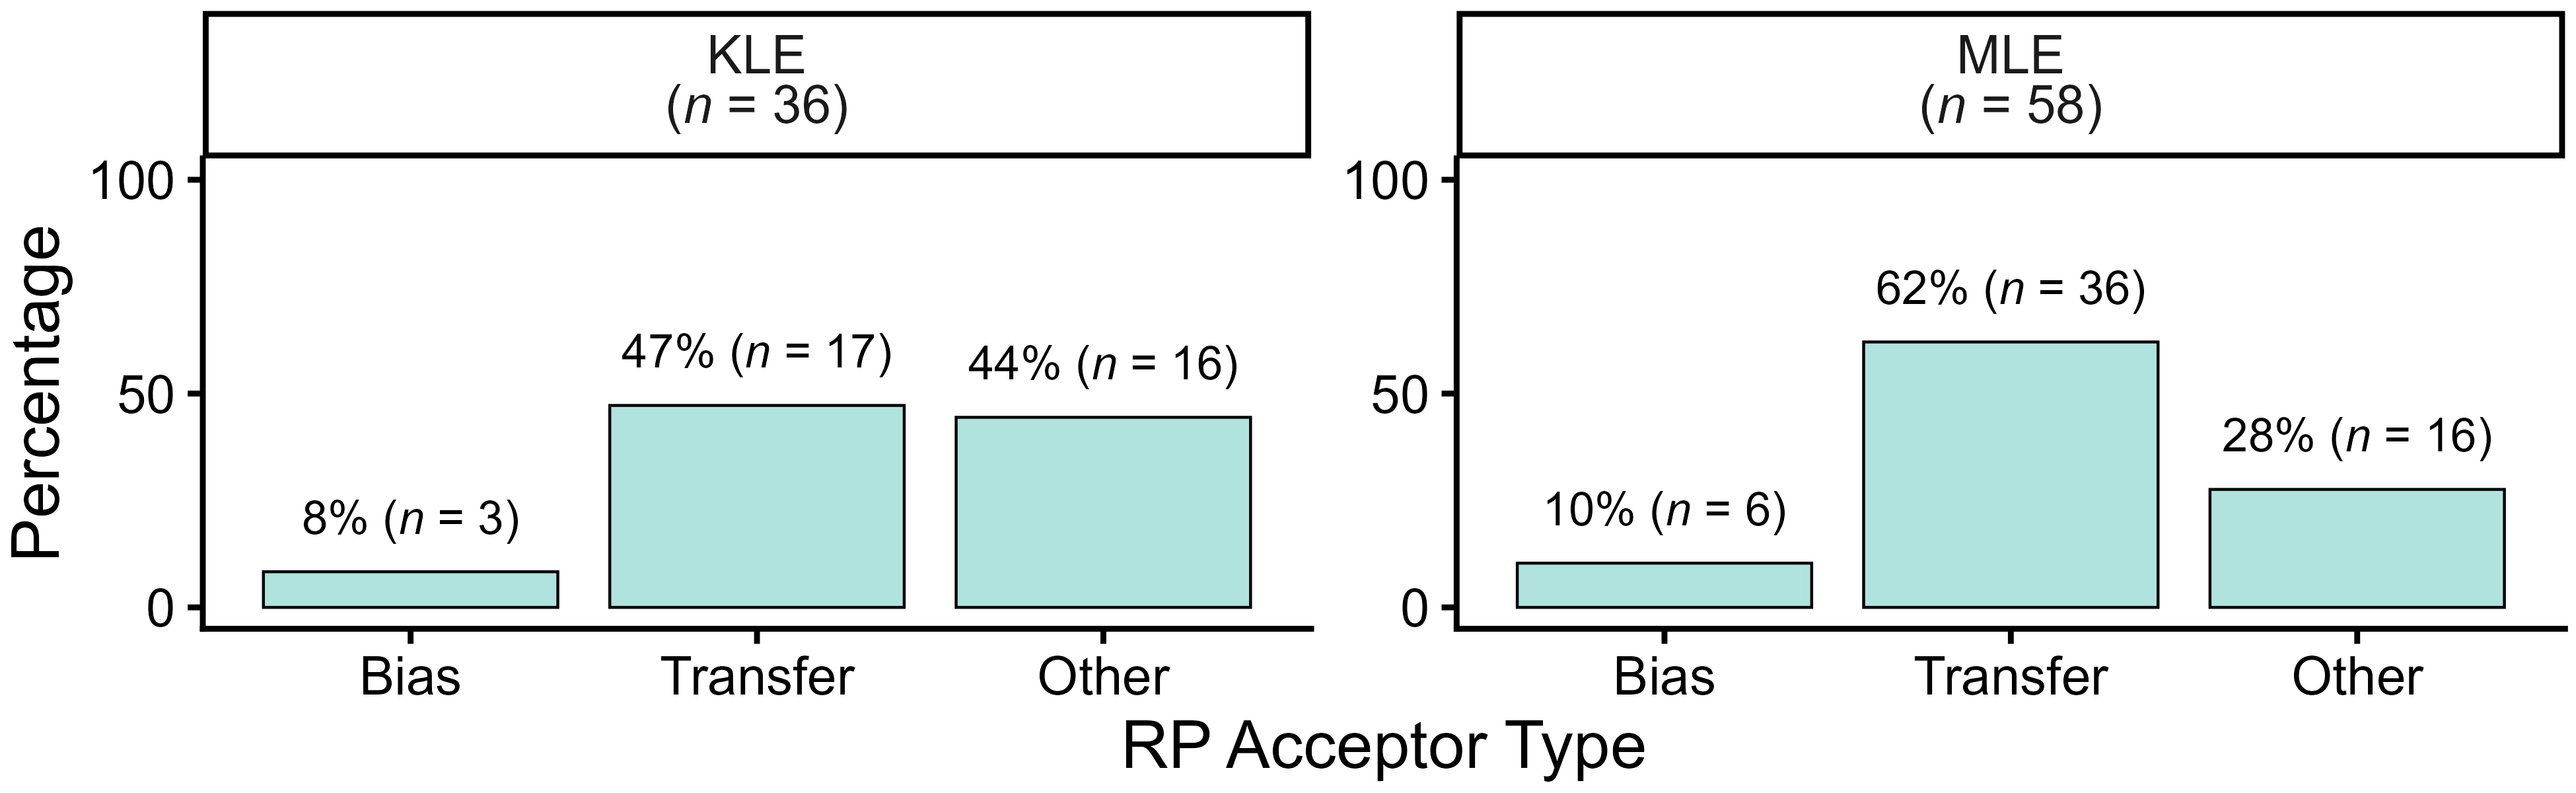
\includegraphics{../analysis/plots/src_ajt_acceptor_type.png}
% \textit{Note}. Values are participant counts with percentages shown in parentheses.
% \vspace{-12pt}
% \end{figure}

% ORC Model (Old)
% \begin{table}
% \caption{Summary of simple linear regression model on L2 proficiency scores for RP acceptors/rejectors in the English ORC acceptability judgment task}\label{tab:app-orc-ajt-acceptor-type-proficiency-model}
% \raggedright\setstretch{1}
% \begin{tabularx}{\textwidth}{lrYYY}\toprule
% Parameter & Estimate~($\hat{\beta}$) & \textit{SE} & $z$ & $p$ \\\midrule
% \csvreader[late after line=\\,late after last line=\\\bottomrule]
% {../analysis/tables/orc_ajt_acceptor_type_proficiency_model.csv}{}{\csvcoli & \csvcolii & \csvcoliii & \csvcoliv & \csvcolv}
% \end{tabularx}
% \textit{Note}. Model formula: Model formula: Proficiency \~{} Group * Type; reference level: KLE + RP Rejector; estimate unit: proficiency $z$-score; intercept: grand mean.
% \vspace{-12pt}
% \end{table}

% SRC Model (Old)
% \begin{table}
% \caption{Summary of simple linear regression model on L2 proficiency scores for RP acceptors/rejectors in the English SRC acceptability judgment task}\label{tab:app-src-ajt-acceptor-type-proficiency-model}
% \raggedright\setstretch{1}
% \begin{tabularx}{\textwidth}{lrYYY}\toprule
% Parameter & Estimate~($\hat{\beta}$) & \textit{SE} & $z$ & $p$ \\\midrule
% \csvreader[late after line=\\,late after last line=\\\bottomrule]
% {../analysis/tables/src_ajt_acceptor_type_proficiency_model.csv}{}{\csvcoli & \csvcolii & \csvcoliii & \csvcoliv & \csvcolv}
% \end{tabularx}
% \textit{Note}. Model formula: Model formula: Proficiency \~{} Group * Type; reference level: KLE + RP Rejector; estimate unit: proficiency $z$-score; intercept: grand mean.
% \vspace{-12pt}
% \end{table}

% ORC Figure (Old)
% \begin{figure}
% \caption{Mean L2 proficiency scores for RP acceptors/rejectors in the English ORC acceptability judgment task} \label{fig:app-orc-ajt-acceptor-type-proficiency}
% \raggedright\setstretch{1}
% 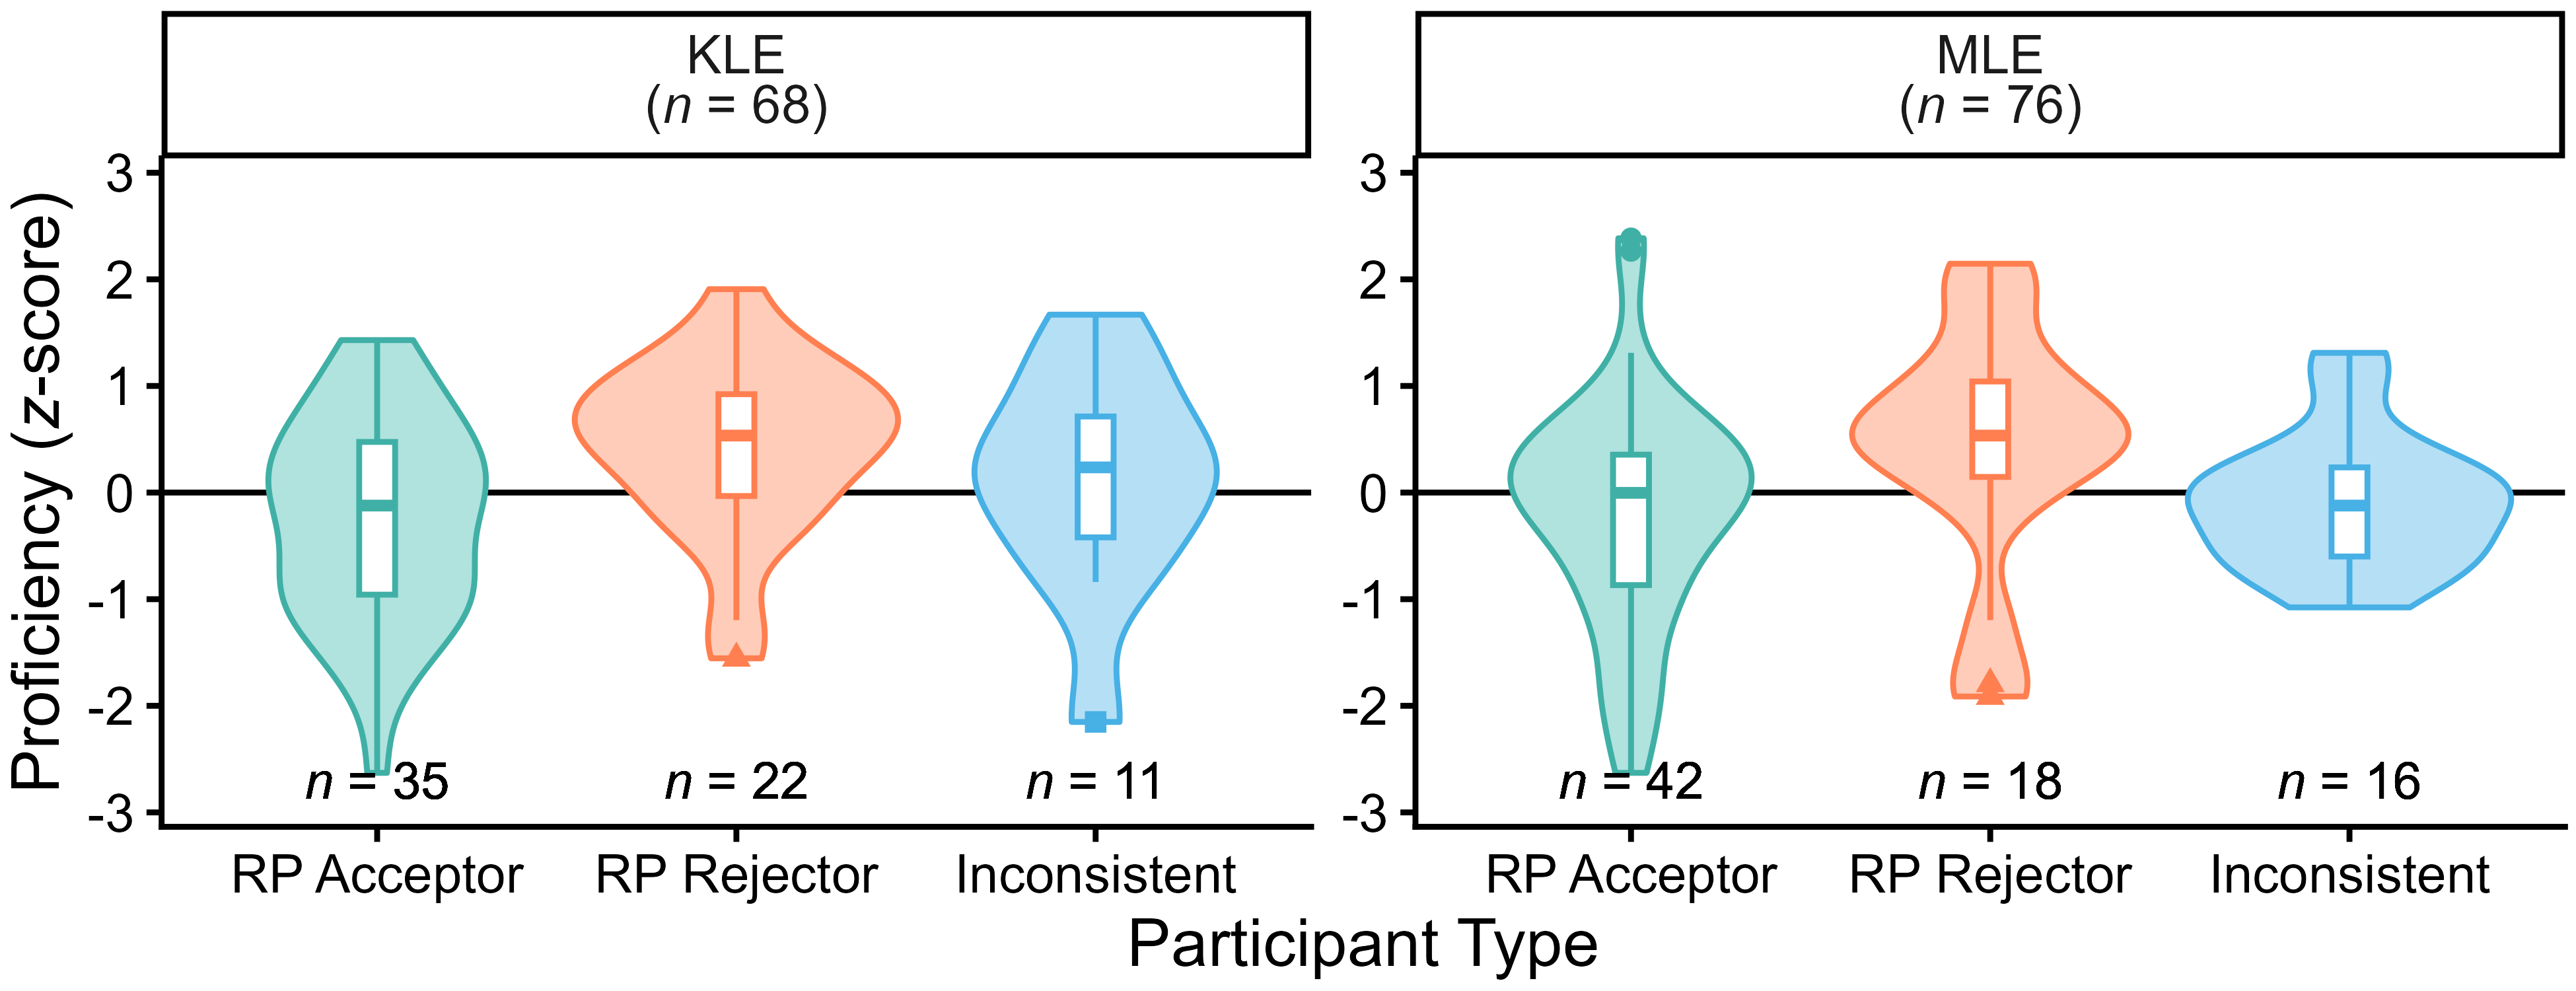
\includegraphics{../analysis/plots/orc_ajt_acceptor_type_proficiency.png}
% \textit{Note}. Error bars are 95\% \textit{CI}s; the \textit{yes}-bias category of RP acceptors are excluded from these plots.
% \vspace{-12pt}
% \end{figure}

% SRC Figure (Old)
% \begin{figure}
% \caption{Mean L2 proficiency scores for RP acceptors/rejectors in the English SRC acceptability judgment task} \label{fig:app-src-ajt-acceptor-type-proficiency}
% \raggedright\setstretch{1}
% 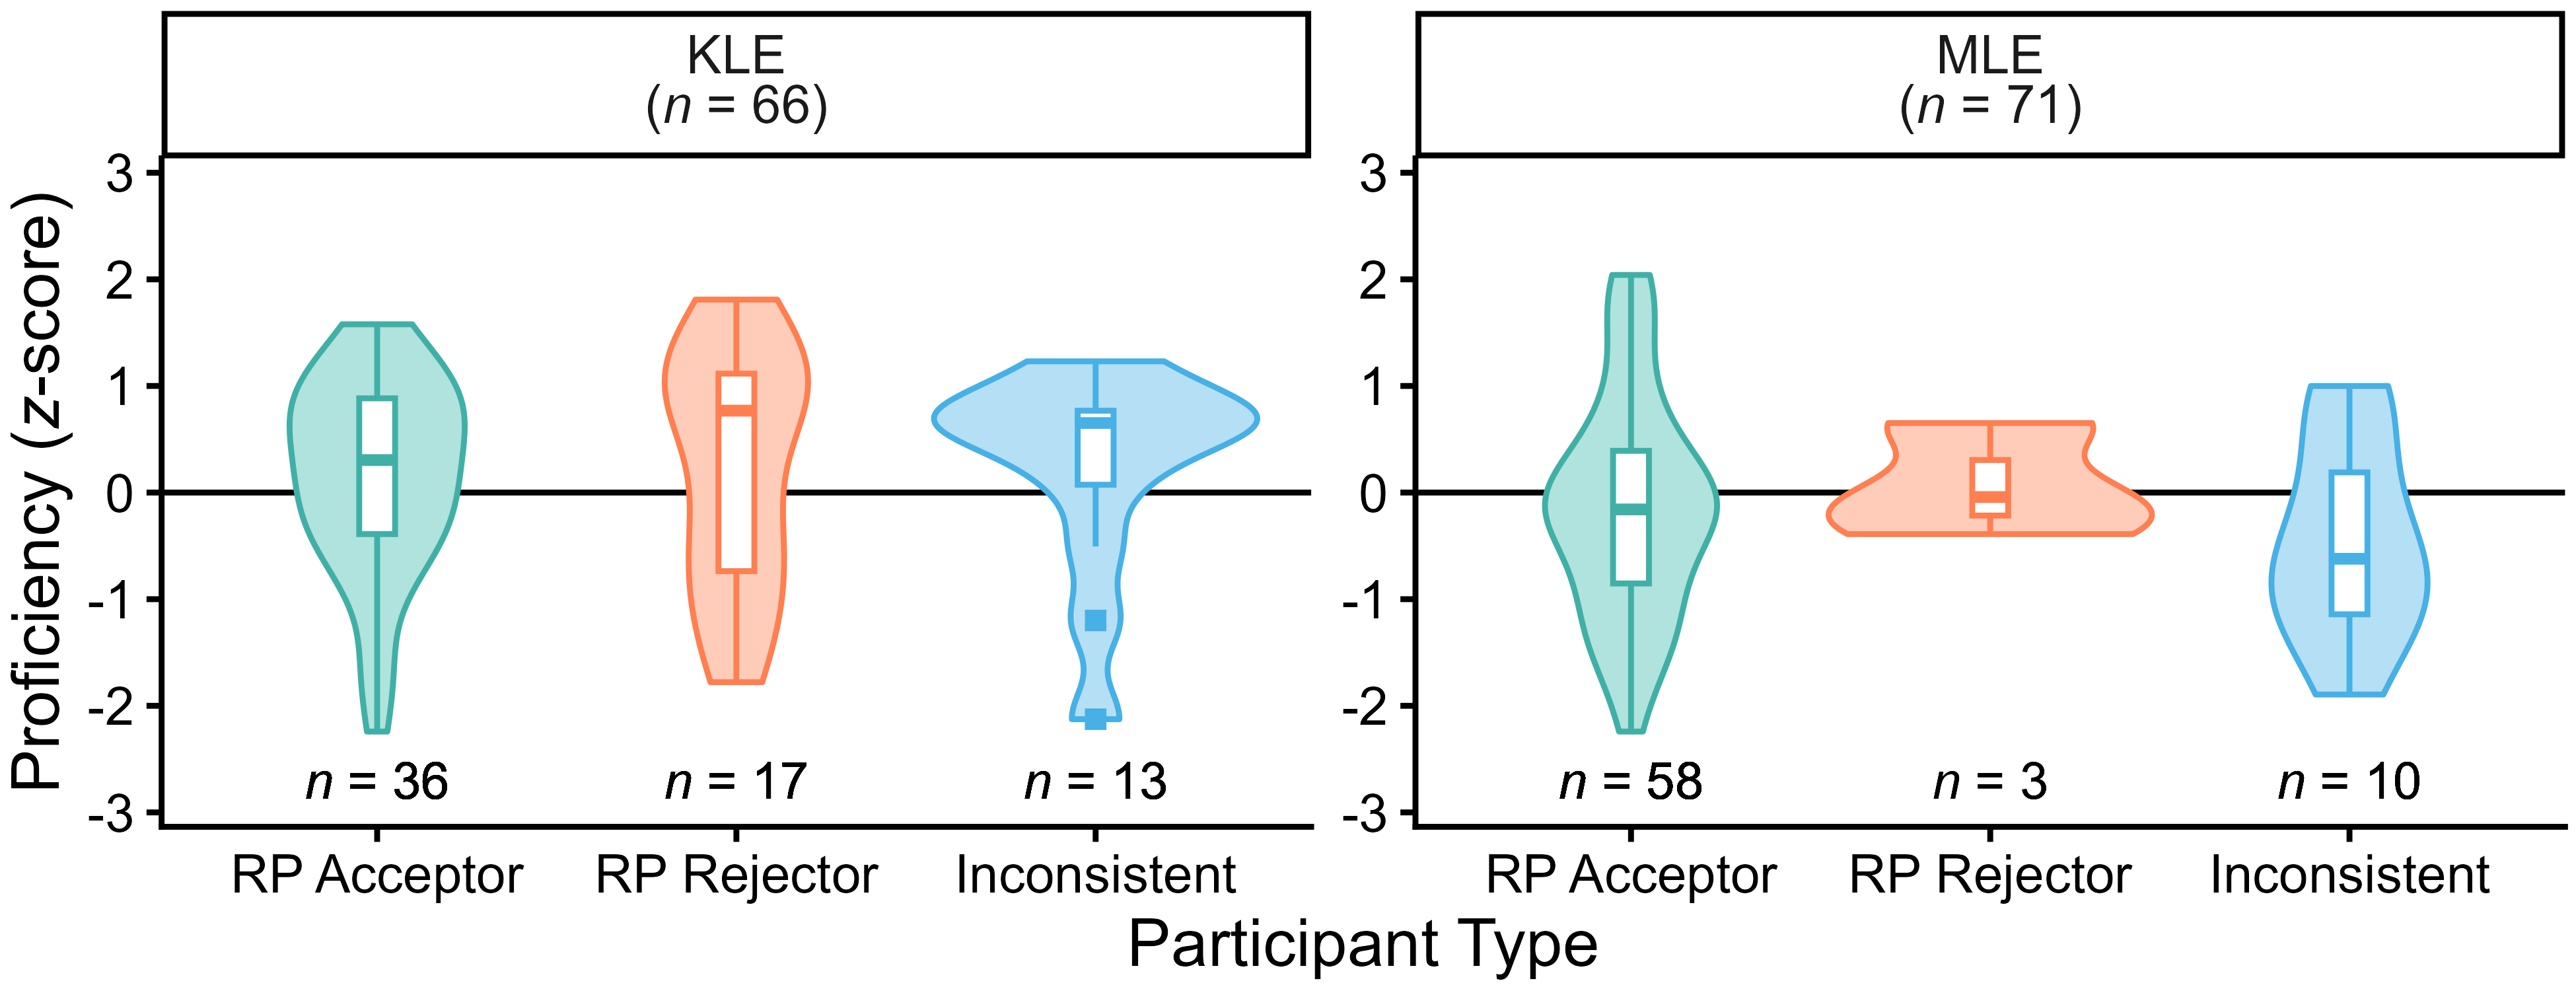
\includegraphics{../analysis/plots/src_ajt_acceptor_type_proficiency.png}
% \textit{Note}. Error bars are 95\% \textit{CI}s; the \textit{yes}-bias category of RP acceptors are excluded from these plots.
% \end{figure}

%========================================================%
\section{Rating patterns for fillers}\label{app-ajt-filler}
%========================================================%

% ORC Means
% \DTLloaddb{dt-ajt-filler-rating}{../analysis/tables/ajt_filler_rating.csv}
% \ExplSyntaxOn
% \tl_clear:N \tblrbody
% \tl_build_begin:N \tblrbody
% \DTLforeach[\equal{\study}{ORC}]{dt-ajt-filler-rating}{\study=study,\coli=Pairing,\colii=Type,\coliii=Grammaticality,\coliv=Mean,\colv=$CI$}{\tl_build_put_right:Ne \tblrbody {\exp_not:V \coli & \exp_not:V \colii & \exp_not:V \coliii & \exp_not:V \coliv & \exp_not:V \colv\\}}
% \tl_build_end:N \tblrbody
% \ExplSyntaxOff
% \begin{longtblr}[caption={Mean ratings for fillers in the ORC acceptability judgment task}, label={tblr:app-orc-ajt-filler-rating}, expand=\tblrbody]{colspec={XXXX[r]X[r]}}\toprule
% Pairing & Type & Grammaticality & Mean & 95\% \textit{CI}\\\midrule
% \tblrbody\bottomrule
% \end{longtblr}
% \vspace{-12pt}

% SRC Means
% \ExplSyntaxOn
% \tl_clear:N \tblrbody
% \tl_build_begin:N \tblrbody
% \DTLforeach[\equal{\study}{SRC}]{dt-ajt-filler-rating}{\study=study,\coli=Pairing,\colii=Type,\coliii=Grammaticality,\coliv=Mean,\colv=$CI$}{\tl_build_put_right:Ne \tblrbody {\exp_not:V \coli & \exp_not:V \colii & \exp_not:V \coliii & \exp_not:V \coliv & \exp_not:V \colv\\}}
% \tl_build_end:N \tblrbody
% \ExplSyntaxOff
% \begin{longtblr}[caption={Mean ratings for fillers in the SRC acceptability judgment task}, label={tblr:app-src-ajt-filler-rating}, expand=\tblrbody]{colspec={XXXX[r]X[r]}}\toprule
% Pairing & Type & Grammaticality & Mean & 95\% \textit{CI}\\\midrule
% \tblrbody\bottomrule
% \end{longtblr}
% \vspace{-12pt}

% ORC Figure
\begin{figure}
\caption{Mean ratings for fillers in the ORC acceptability judgment tasks} \label{fig:app-orc-ajt-filler-rating}
\raggedright\setstretch{1}
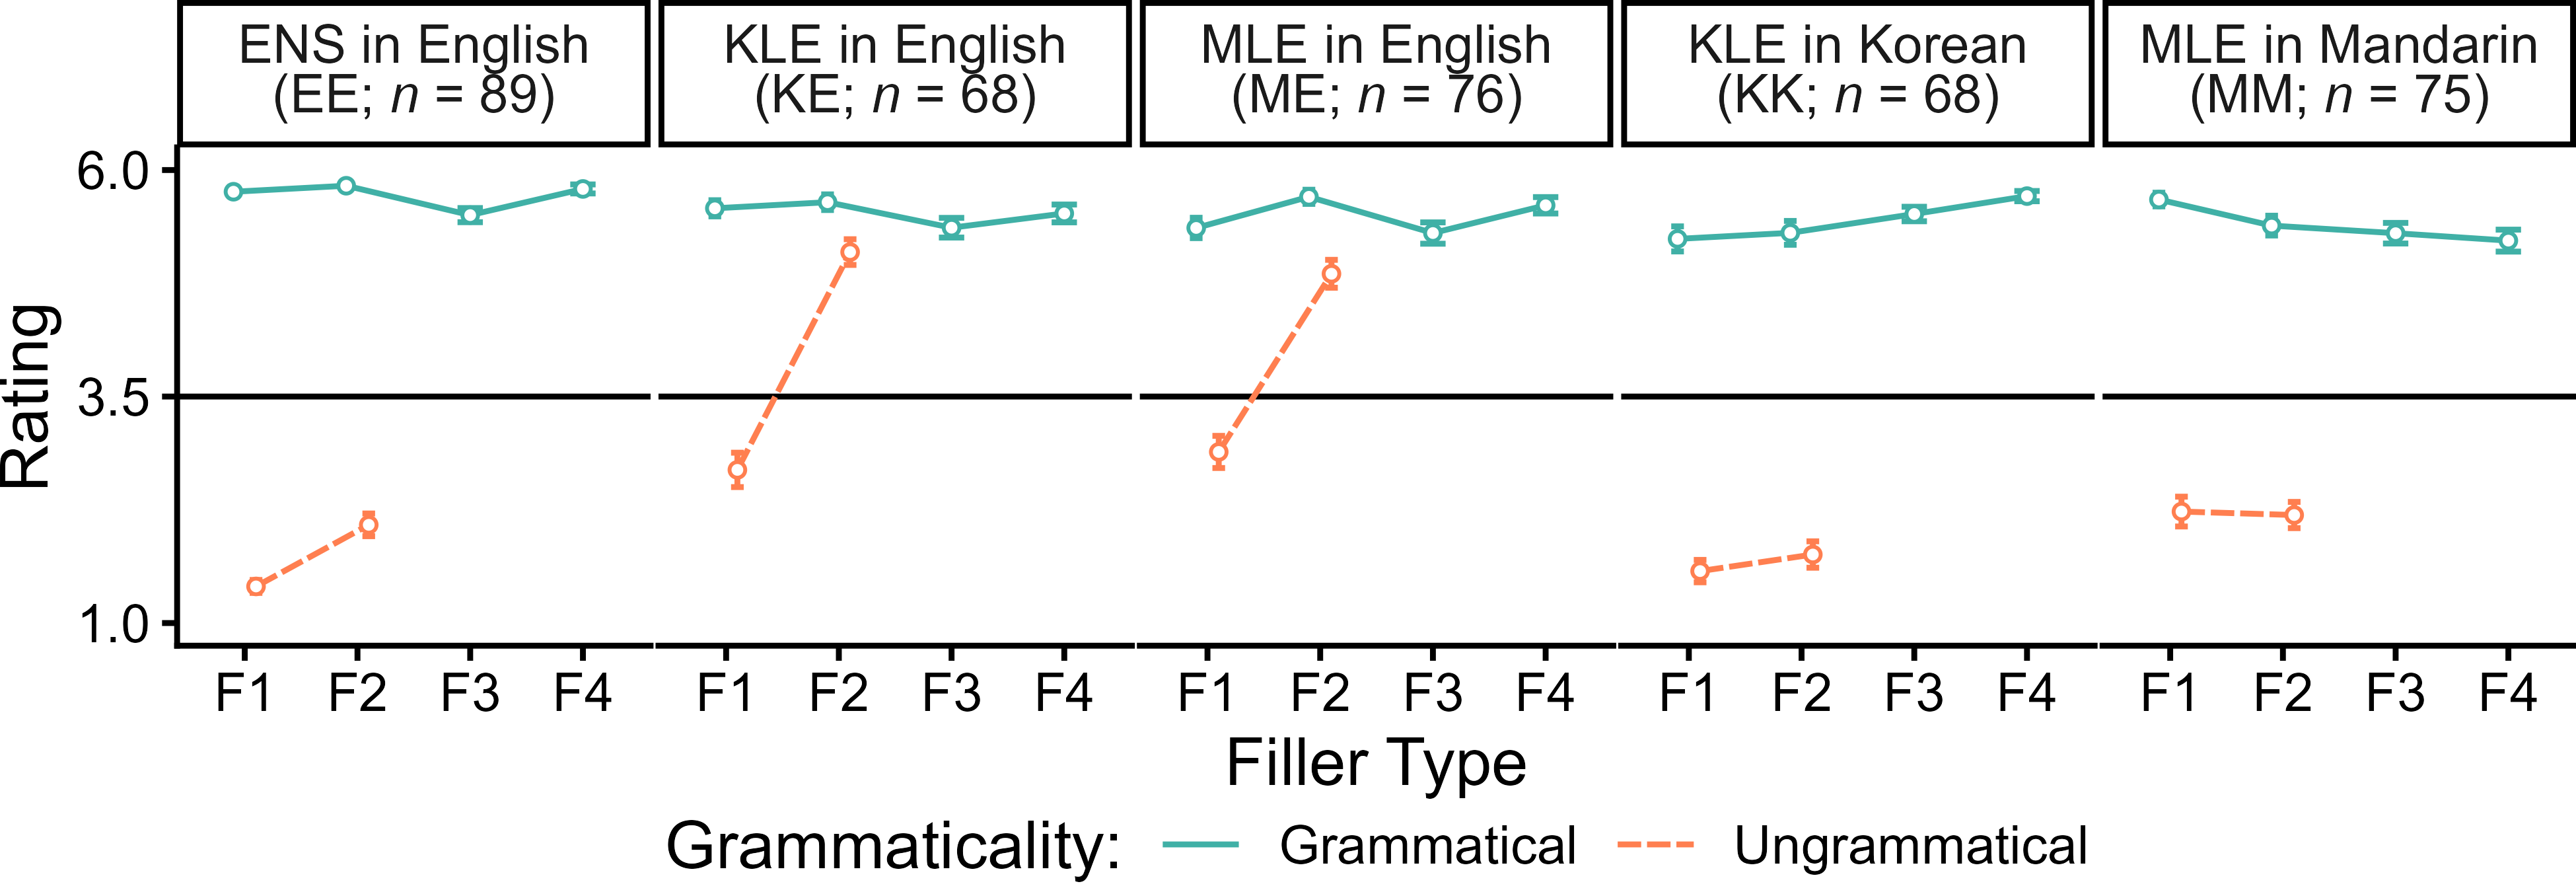
\includegraphics{../analysis/plots/orc_ajt_filler_rating.png}
\textit{Note}. Error bars are 95\% \textit{CI}s.
\vspace{-12pt}
\end{figure}

% SRC Figure
\begin{figure}
\caption{Mean ratings for fillers in the SRC acceptability judgment tasks} \label{fig:app-src-ajt-filler-rating}
\raggedright\setstretch{1}
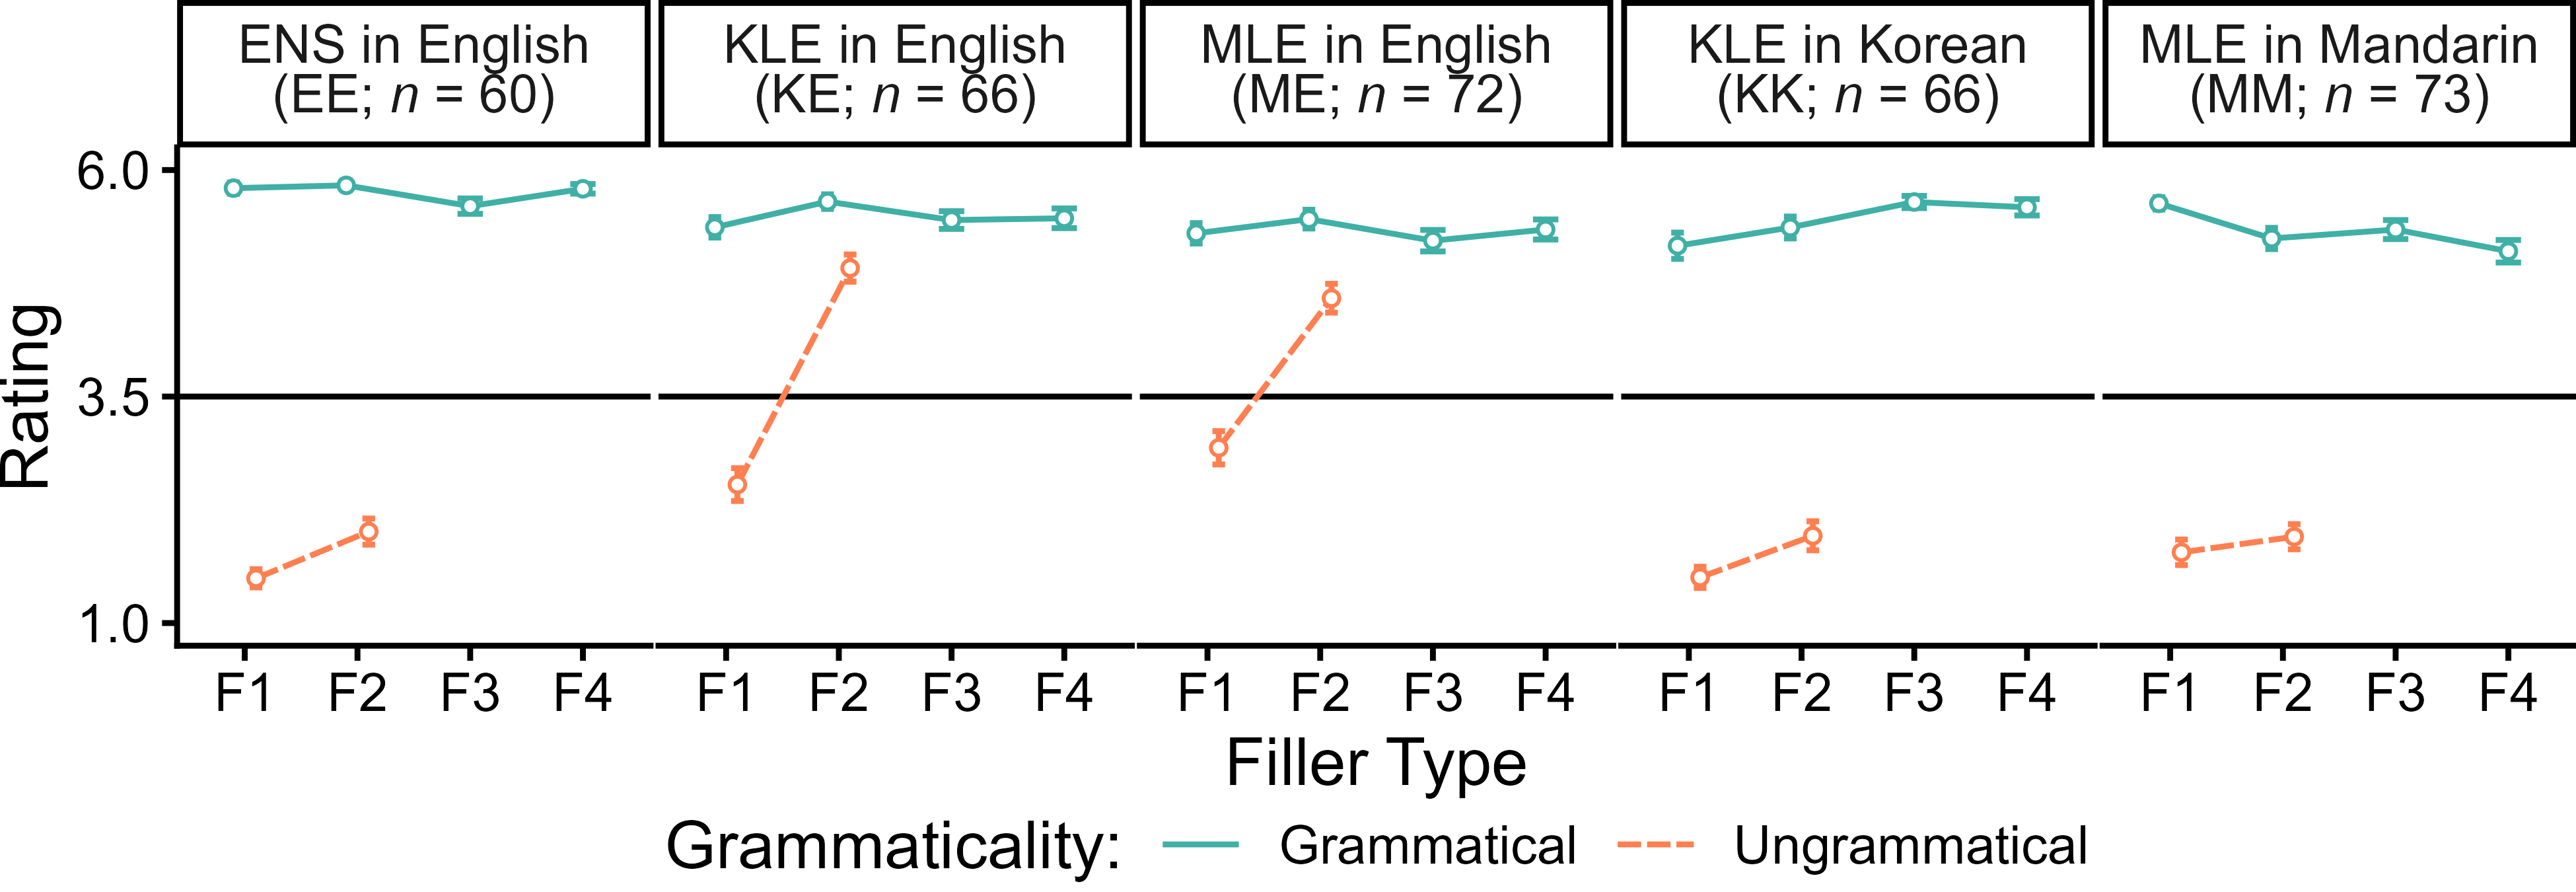
\includegraphics{../analysis/plots/src_ajt_filler_rating.png}
\textit{Note}. Error bars are 95\% \textit{CI}s.
\vspace{-12pt}
\end{figure}